\chapter{Methodology and System Design}
\label{ch:methodology}

This chapter describes the empirical infrastructure --- datasets, the detection-scoring rule, scoring-rule and data-leakage audits, and the reproducibility layer --- and then, building on it, the system architecture and component designs (\S\ref{ch:architecture}).

\section{Datasets}
\label{sec:datasets}

The evaluation uses seven labelled corpora and a 19-clip YouTube real-video set, drawn from public benchmarks, Roboflow / Kaggle sources, and the deployment partner's CCTV stream. Full provenance is in Appendix~\ref{app:datasets}.

\begin{table}[htbp]
    \centering
    \caption{Top-level evaluation surfaces used in this thesis. ``Role'' indicates whether the corpus is a training surface, an in-distribution evaluation surface, an OOD evaluation surface, or all three.}
    \label{tab:datasets}
    \begin{tabular}{lrlp{5.6cm}}
        \toprule
        Tag & Frames & Modality & Role \\
        \midrule
        \texttt{rgb\_dataset} (composite RGB corpus) & 172,022 & RGB & RGB-detector train + in-distribution test \\
        \texttt{ir\_dset\_final} & 129,130 & IR & IR-detector train + in-distribution test \\
        \texttt{rgb\_confusers\_merged} & 27,024 & RGB & Confuser hard-negative training source + OOD confuser-zoo test (test split 2{,}633) \\
        \texttt{svanstrom} (paired) & 28,710 & RGB+IR & Discriminating benchmark (small drones; labelled confusers) \\
        \texttt{antiuav} (RGBT) & 85,374 & RGB+IR & Saturated benchmark / sanity floor \\
        \texttt{selcom\_cctv} & 2,076 & RGB & Deployment-partner CCTV (fine-tune surface) \\
        Roboflow nine-set OOD audit & --- & RGB + IR & OOD generalisation audit \\
        YouTube real-video diagnostic & $\approx$2{,}484 sampled & RGB & Real-world drone-positive (9) + confuser-only (10) clips \\
        \bottomrule
    \end{tabular}
\end{table}

\begin{figure}[htbp]
    \centering
    
\includegraphics[width=0.92\textwidth]{fig_dataset_montage}
    \caption{Ground-truth drone crops across datasets and modalities (red box $=$ GT; window $\approx 4\times$ the box). Svanstr\"om drones are $19$--$29$~px small silhouettes against open sky --- the regime that makes birds and distant aircraft hard to separate and that drives the cascade --- while Anti-UAV drones are an order of magnitude larger; the thermal (IR) view renders the same target as a bright blob rather than a dark silhouette (\S\ref{sec:design_rationale}).}
    \label{fig:dataset_montage}
\end{figure}

\subsection{Composite RGB Training Corpus (\texttt{rgb\_dataset})}
\label{sec:ds_rgb_corpus}

The RGB detector's training and in-distribution test corpus is a composite of nine public sources totalling 172{,}022 frames split 80/10/10 (137{,}506 train, 17{,}307 val, 17{,}209 test), sequence-disjoint. Of these, 134{,}339 (78.1\%) carry at least one drone box and 37{,}683 (21.9\%) are background negatives; the corpus contains 146{,}540 drone-class boxes. Per-source breakdown:
% [source: dataset=rgb_dataset; file=rgb_dataset/dataset.yaml (filename-prefix manifest)]

\begin{table}[htbp]
    \centering
    \caption{Per-source composition of the composite RGB training corpus. Negatives include VIRAT surveillance, UA-DETRAC traffic, and BDD100K driving frames as background contrast.}
    \label{tab:ds_rgb_components}
    \begin{tabular}{lrp{7.2cm}}
        \toprule
        Source prefix & Count & Description \\
        \midrule
        \texttt{anti}                 & 59{,}413 & Anti-UAV benchmark (CVPR 2020 / 2021)~\cite{jiang2021antiuav} RGB frames \\
        \texttt{wosdetc}              & 53{,}259 & WosDetC drone corpus \\
        \texttt{anti-muav-roboflow}   & 14{,}652 & Anti-mUAV Roboflow community variant \\
        \texttt{AirBird}              & 10{,}000 & AirBird drone-vs-bird dataset (supplies bird negatives at training time) \\
        \texttt{FBD-SV}               &  9{,}754 & Fine-grained Bird Detection (Sky View) \\
        \texttt{mav}                  &  9{,}744 & MAV (Micro Aerial Vehicle) frames \\
        \texttt{dut}                  &  5{,}200 & DUT aerial imagery \\
        \texttt{VIRAT}                &  3{,}334 & VIRAT surveillance benchmark (background negatives) \\
        \texttt{UA-DETRAC}            &  3{,}333 & UA-DETRAC traffic benchmark (background negatives) \\
        \texttt{BDD100K}              &  3{,}333 & BDD100K driving dataset (background negatives) \\
        \midrule
        \textbf{Total}                & \textbf{172{,}022} & 80/10/10 split; \texttt{drone} is the only positive class \\
        \bottomrule
    \end{tabular}
\end{table}

The \texttt{AirBird} subset supplies the bird hard negatives that make the baseline meaningful rather than a strawman. Svanstr\"om frames appear only as \texttt{DRONE} training positives; the bird / airplane / helicopter splits are absent and therefore OOD for the baseline at evaluation time.

\subsection{Confuser Hard-Negative Corpus (\texttt{rgb\_confusers\_merged})}
\label{sec:ds_confusers}

The hard-negative training source for the \texttt{hardneg\_v3more} and \texttt{retrained\_v2} variants, and the OOD confuser-zoo test split. 27{,}024 images, all with empty YOLO labels, from seven sources split 80/10/10 (21{,}784 train, 2{,}607 val, 2{,}633 test). Sources without existing splits were divided by video / sequence ID to prevent temporal leakage (Svanstr\"om: 165 sequences; raihanrsd Kaggle: 58 folders; Helicopter Kaggle: hash-based pseudo-groups).

\begin{table}[htbp]
    \centering
    \caption{Per-source composition of the RGB confuser hard-negative corpus. The test split (right column) is the \emph{OOD confuser zoo} evaluation surface used in Section~\ref{ch:experiments}.}
    \label{tab:ds_confusers}
    \begin{tabular}{llrrr}
        \toprule
        Source & Category & Train & Val & Test \\
        \midrule
        Svanstr\"om paired & Airplane    & 4{,}528 &   528 & 1{,}034 \\
        Svanstr\"om paired & Helicopter  & 4{,}489 &   827 &    311 \\
        Svanstr\"om paired & Bird        & 4{,}586 &   303 &    409 \\
        New\_Dataset (Roboflow) & Mixed  & 3{,}514 &   439 &    439 \\
        Airplane (Roboflow) & Airplane   & 2{,}093 &   200 &     99 \\
        Helicopter (Kaggle) & Helicopter & 1{,}387 &   188 &    175 \\
        raihanrsd (Kaggle) & Bird        & 1{,}187 &   122 &    166 \\
        \midrule
        \textbf{Total}     &             & \textbf{21{,}784} & \textbf{2{,}607} & \textbf{2{,}633} \\
        \bottomrule
    \end{tabular}
\end{table}

Ten airplane / Roboflow frames containing visible drones were removed during curation. Hard-negative mining for \texttt{retrained\_v2} (\S\ref{sec:rgb_three_variants}) ran the baseline detector over all 27{,}024 confuser images, retained the 11{,}729 (43.4\%) on which it hallucinated, and merged those with the composite RGB corpus to produce the 183{,}751-image \texttt{retrain\_dataset}.
% [source: dataset=rgb_confusers_merged; file=rgb_confusers_merged/dataset_documentation.md (hard-negative mining stat)]

\subsection{IR Detector Corpus (\texttt{ir\_dset\_final})}
\label{sec:ds_ir}

129{,}130 thermal frames split 83.5 / 9.1 / 7.4 (107{,}809 train, 11{,}709 val, 9{,}612 test); 72.5\% positive / 27.5\% negative (94{,}142 drone-class boxes). Single-class (\texttt{drone}). Sources by filename prefix:
% [source: dataset=ir_dset_final; file=IR_dset_final/dataset.yaml]

\begin{table}[htbp]
    \centering
    \caption{Per-source composition of \texttt{ir\_dset\_final}. The Svanstr\"om IR partition (\texttt{svan}) is the largest single source and is the reason Svanstr\"om IR evaluation in Section~\ref{ch:experiments} is in-distribution for the IR detector (Table~\ref{tab:svanstrom_audit}).}
    \label{tab:ds_ir_components}
    \begin{tabular}{lrp{7.2cm}}
        \toprule
        Prefix & Count & Description \\
        \midrule
        \texttt{dv5}    & 53{,}512 & DV5 thermal drone sequences \\
        \texttt{cst}    & 22{,}957 & CST thermal captures \\
        \texttt{svan}   & 21{,}637 & Svanstr\"om IR drone partition \\
        \texttt{czoom}  &  9{,}808 & CZoom thermal zoom sequences (train only) \\
        \texttt{sea}    &  8{,}398 & Sea / maritime thermal backgrounds (negatives) \\
        \texttt{flir}   &  6{,}360 & FLIR thermal imagery \\
        \texttt{ovh2}   &  2{,}898 & Overhead thermal set 2 \\
        \texttt{ovh1}   &  2{,}866 & Overhead thermal set 1 \\
        \texttt{gemini} &     392 & Gemini thermal captures (synthetic-augmented) \\
        \texttt{yt}     &     302 & YouTube thermal clips (train only) \\
        \midrule
        \textbf{Total}  & \textbf{129{,}130} & 83.5 / 9.1 / 7.4 split; 72.5\% positive / 27.5\% negative \\
        \bottomrule
    \end{tabular}
\end{table}

Bird, airplane, and helicopter thermal frames enter across HITL revisions (\S\ref{sec:hitl_ir}) as the IR detector hallucinates on confuser scenes; \texttt{sea} and sky/building negatives are similarly mined. This state corresponds to the production \texttt{v3b} checkpoint; earlier revisions (V2--V5) operated on smaller variants of the same source families.

\subsection{Svanstr\"om Paired (\texttt{svanstrom})}
\label{sec:ds_svanstrom}

The Svanstr\"om dataset~\cite{svanstrom2021real,svanstrom2022dronedataset} is the discriminating benchmark. The paired version contains 28{,}710 frames at stride~3 from 279 sequences, at $640{\times}512$ native resolution. Drones are routinely a few tens of pixels across --- the regime driving the imgsz~640 vs.~1280 swing of Figure~\ref{fig:resolution}. Per-class counts: 11{,}695 drone, 6{,}090 airplane, 5{,}298 bird, 5{,}627 helicopter. Svanstr\"om RGB scoring uses IoP at 0.5 (\S\ref{sec:metrics}) because annotators drew loose boxes and IoU systematically under-counts useful predictions.

\subsection{Anti-UAV RGBT (\texttt{antiuav})}
\label{sec:ds_antiuav}

The Anti-UAV RGBT benchmark~\cite{jiang2021antiuav,zhao2023antiuav} provides large-scale paired RGB+IR sequences ($1920{\times}1080$ RGB, $640{\times}512$ IR). Both modalities saturate at $F1 \geq 0.99$ (RGB) and $\geq 0.96$ (IR) on the 85{,}374 evaluated frames. Anti-UAV is a sanity floor: a strong result here is necessary but not sufficient; Svanstr\"om and the real-video diagnostic do the discriminating work.
% [source: ledger=antiuav-saturated; eval=rgb_antiuav_baseline; run=eval/ablate.py; cache=eval/results/_ablation/2026-05-18T22-48-19/master.csv; config=antiuav_iou_1280_s5]

\subsection{SelCom CCTV (\texttt{selcom\_cctv})}
\label{sec:ds_selcom}

The deployment-partner corpus: a fixed-camera 7~Mbps HEVC stream (\texttt{yuvj420p}, $1920{\times}1080$, 25~fps, $\sim$1:30) covering an urban perimeter. 2{,}076 frames (1{,}953 drone-positive + 123 true negatives), median drone $\sqrt{\text{area}} \approx 36.8$~px ($\sim$12~px at \texttt{imgsz=640}, $\sim$24~px at 1280). Drones blend into urban clutter, making SelCom a clutter-bound rather than purely pixel-bound regime. The \texttt{selcom\_mixed\_ft2\_val} surface (311 images, 295 GT boxes) is a pure-SelCom 15\% held-out split (seed~0); the SelCom fine-tune \texttt{Yolo26n\_selcom\_mixed\_ft2\_1280} (\S\ref{sec:selcom_finetune}; a comparison detector --- the shipped RGB detector is \texttt{ft4}, \S\ref{sec:training_recipes}) trains on the remaining frames mixed 20:80 with general RGB.
% [source: dataset=selcom_cctv; file=SelCom CCTV manifest (see \S\ref{sec:ds_selcom})]

\subsection{Roboflow OOD Audit (Nine Datasets)}
\label{sec:ds_roboflow}

A targeted OOD audit from nine Roboflow / Kaggle datasets characterising RGB and IR detectors off-distribution (\S\ref{sec:roboflow}): three RGB-drone splits (\texttt{rgb\_drone\_*}), three RGB-confuser splits (airplane, bird, helicopter), and three IR splits (\texttt{ir\_drone\_night}, \texttt{ir\_mixed\_cbam}, IR airplane / bird). Per-split counts are in Appendix~\ref{app:datasets}. No dataset here is used for training.

\subsection{YouTube Real-Video Diagnostic (19 Clips)}
\label{sec:ds_youtube}

19 curated YouTube clips totalling $\approx$2{,}484 sampled frames: 9 drone-positive (1{,}234 GT drone instances, several with concurrent birds) and 10 confuser-only (1{,}250 frames; every detection is a false positive). The drone-positive set was annotated frame-by-frame; stride was set to yield $\sim$20--340 frames per clip. The full per-clip table is in Appendix~\ref{app:datasets}.

This is the only fully OOD surface for every cascade component: no clip appears in any training set, imagery is consumer-grade, and the drone-positive clips include bird-vs-drone scenes absent from Svanstr\"om.

\begin{figure}[htbp]
    \centering
    
\includegraphics[width=0.8\textwidth]{fig_drone_size_hist}
    \caption{Drone size in native pixels (sampled GT boxes). Svanstr\"om drones cluster at the YOLOv26n small-object floor --- a large fraction fall below the \texttt{imgsz=640} resolvable size ($\sqrt{\text{area}}\approx 8$~px) but above the \texttt{imgsz=1280} floor ($\approx 4$~px), which is why Svanstr\"om recall collapses at \texttt{imgsz=640} and resolves at \texttt{imgsz=1280} (\S\ref{sec:resolution_arch}); Anti-UAV drones are an order of magnitude larger and supra-floor at either resolution.}
    \label{fig:drone_size_hist}
\end{figure}

\begin{figure}[htbp]
    \centering
    
\includegraphics[width=0.85\textwidth]{fig_confuser_panel}
    \caption{The confuser problem, and why a downstream filter solves it. \emph{Left}: the production RGB detector (\texttt{ft4}) fires on a bird amid its flock (red box, detector confidence $0.46$). \emph{Right}: it fires on a drone (confidence $0.85$). The detector cannot tell them apart --- but the feature-reuse verifier reads the detector's own ROI features and assigns $P(\text{drone})=0.00$ to the bird (vetoed) and $0.96$ to the drone (kept). This separation, not a better detector, is what the cascade provides.}
    \label{fig:confuser_problem}
\end{figure}

\section{Metrics and the IoP Rule}
\label{sec:metrics}

Detection scoring uses \textbf{Intersection over Prediction (IoP)} at threshold 0.5 for all Svanstr\"om RGB scoring:
\[
\text{IoP} = \frac{|B_\text{pred} \cap B_\text{gt}|}{|B_\text{pred}|}
\]
A prediction is a true positive iff $\text{IoP} \geq 0.5$ against some GT box; otherwise it is a false positive. IoP is used because Svanstr\"om GT boxes are routinely larger than the drone, so IoU systematically under-counts useful predictions. Anti-UAV uses standard IoU; GT boxes are tight and IoU/IoP differ negligibly.

The headline metrics are \emph{precision}, \emph{recall}, and \emph{F1}; mAP50 and mAP50-95 appear only as supplementary numbers (e.g., Table~\ref{tab:ir_evolution}). Precision and recall directly reflect false-alarm and missed-drone rates; a single mAP obscures both. For confuser-only surfaces the headline is \emph{fire rate} or \emph{FPPI}, since no drone GT exists.

\subsection{Scoring-Rule Sensitivity}
\label{sec:scoring_audit}

A methodological caveat concerns how a multi-modal detection is scored. Under \emph{dual scoring}, each modality is scored independently and FN/FP counts aggregated, so a frame silent on RGB but detected on IR still books an RGB FN. Under \emph{trust-aware scoring}, only the modality the trust classifier chose is scored. The user sees one per-frame alert; trust-aware scoring matches that; dual scoring does not.

On Svanstr\"om the same detections move by $27.7$~pp: dual scoring gives $F1=0.663$ (recall $0.501$) vs.\ trust-aware $F1=0.940$ (recall $0.904$) at identical precision ($0.979$). All cascade-level F1 in this thesis uses trust-aware scoring unless noted; any cross-paper comparison of multi-modal $F1$ must state its scoring rule.
% [source: ledger=scoring-rule-swing; run=(May-10 ablation, E_scoring branch); cache=eval/results/_ablation/2026-05-10T16-08-14/master.csv; config=svan_iop_640_may10]

\section{Svanstr\"om Usage Audit}
\label{sec:svanstrom_audit}

Svanstr\"om appears in both training and evaluation for some components; the leakage risk is made explicit below.

\begin{table}[htbp]
    \centering
    \caption{Svanstr\"om data appearance per component. The trust classifier has the most material overlap; Anti-UAV is fully clean and is used as the mitigation.}
    \label{tab:svanstrom_audit}
    \begin{tabular}{lccl}
        \toprule
        Component & In training? & In eval? & Notes \\
        \midrule
        RGB detector  & No  & Yes (28,710) & Genuine OOD for the RGB model \\
        IR detector   & Yes (21{,}637 frames) & Yes (28,710) & \texttt{svan} prefix in \texttt{IR\_dset\_final/train} \\
        Trust classifier & Yes (frames) & Yes (28,710) & Sequence-stratified split; eval on full set \\
        Patch verifier & No & Yes (crops) & Clean \\
        \bottomrule
    \end{tabular}
\end{table}

The group-shuffled split prevents within-classifier temporal leakage but not cascade-level evaluation on classifier-training sequences. Svanstr\"om classifier numbers are in-distribution and should be read as upper bounds. Anti-UAV cascade numbers are fully clean, and production decisions in Section~\ref{ch:architecture} are anchored on Anti-UAV results.

\section{Training Recipes}
\label{sec:training_recipes}

All detectors are YOLOv26n (nano) single-class drone detectors; the IR detector's per-revision configuration is in \S\ref{sec:hitl_ir}.

\begin{table}[htbp]
    \centering
    \caption{Detector training configurations. The baseline RGB and \texttt{retrained\_v2} share a recipe but differ in training corpus (\S\ref{sec:rgb_three_variants}). All training was on an NVIDIA RTX 3090 (24~GB VRAM); evaluation was on a GTX 1050 Ti (4~GB VRAM).}
    \label{tab:training_recipes}
    \begin{tabular}{lcc}
        \toprule
        Parameter & RGB (baseline / \texttt{retrained\_v2}) & SelCom fine-tune (\texttt{ft2\_1280}) \\
        \midrule
        Pretrained init   & \texttt{yolo26n.pt} (COCO) & \texttt{Yolo26n\_trained} (baseline)        \\
        Epochs            & 70                         & up to 50 with patience~10                   \\
        Patience          & 10                         & 10                                          \\
        Batch size        & 48                         & 4                                           \\
        \texttt{imgsz}    & 640                        & 1280                                        \\
        Optimiser         & AdamW                      & AdamW                                       \\
        Initial LR        & 0.001                      & 0.001                                       \\
        Final LR ratio    & 0.01                       & 0.01                                        \\
        Warmup            & 3 epochs                   & 3 epochs                                    \\
        Weight decay      & 0.0005                     & 0.0005                                      \\
        Mosaic            & 0.33 (off after epoch 50)  & 0.33                                        \\
        Erasing           & 0.4                        & 0.4                                         \\
        Scale / Translate / Flip-LR & 0.5 / 0.1 / 0.5  & 0.5 / 0.1 / 0.5                             \\
        HSV (H, S, V)     & 0.015 / 0.7 / 0.4          & 0.015 / 0.7 / 0.4                           \\
        \bottomrule
    \end{tabular}
\end{table}

\paragraph{Backbone-freeze depth in confuser-injection fine-tuning.}
Injecting hard-negative confuser crops risks catastrophic forgetting. For FT4 --- the feature source for the distilled verifier (\S\ref{sec:distill_verifier}) --- backbone-freeze depth is the controlling knob: freezing 15 layers cleared every drone-recall regression gate, whereas freezing only 12 regressed Svanstr\"om recall and $F1$ at the same $300$ hard negatives. The production recipe (FT4 R3: $300$ hard negatives, \texttt{freeze}$=15$, $3$ epochs) was the only configuration that cleared all gates (R1/R2 failed recall; A1--A4 ratio variants all failed), achieving a $16$-pp confuser-hallucination cut without recall loss.
% [source: ledger=ft4-backbone-freeze]
% [source: ledger=ft4-backbone-freeze; eval=none (regression-gate sweep); run=scripts/auto_confuser_ft4.py; config=ft4]

\section{Reproducibility Infrastructure}
\label{sec:reproducibility}

Every run writes a \texttt{manifest.json} recording: git commit hash; SHA-256 of loaded weights; CUDA version and device; the full command line; per-frame conf threshold and \texttt{imgsz}; and run timestamps. The cache layer (\texttt{eval/cache\_inference.py}) builds a deterministic tag from \texttt{(rgb\_weights\_hash, ir\_weights\_hash, imgsz, stride)}, preventing silent cache reuse across configurations. Every quantitative claim is registered with its source file, reproduction command, and status (\texttt{current} / \texttt{provisional} / \texttt{superseded} / \texttt{placeholder}).

The ablation matrix driver (\texttt{eval/ablate.py}, factor file \texttt{eval/ablations.yaml}) sweeps the cascade's structural axes (RGB model, patch verifier, classifier, cascade, scoring, temporal smoother, grayscale, confidence) and aggregates into \texttt{master.csv} / \texttt{master.md}. The May~10 matrix factors A through H source Table~\ref{tab:cumulative_svanstrom}, the scoring-rule audit, and the cascade comparison. Detector inference is deterministic at fixed weights and conf; the trust classifier (XGBoost) is deterministic at fixed feature input. Only classifier \emph{training} is stochastic, controlled by fixed sequence-stratified group splits.

\section{Model MRI: Feature-Space Analysis}
\label{sec:model_mri}

This thesis follows a \emph{statistics-before-training} discipline: design decisions are settled by measuring what a detector's features encode before any training run. The feature-reuse RGB verifier (\S\ref{sec:distill_verifier}), IR feature separability and grayscale$\leftrightarrow$thermal alignment (\S\ref{sec:ir_xmodal_verifier}), and trust-classifier feature selection (\S\ref{sec:feature_selection}) rest on \emph{feature-space} evidence. That evidence is produced by the \emph{Model MRI} tool (\texttt{python -m mri}; modules \texttt{mri/\{extract,classifier,holdout,modality\}.py}). The tool hooks the detector's FPN layers (\texttt{p3}, stride~8; \texttt{p5}, stride~32) and ROI-pools per-detection activations into a $517$-feature embedding ($512$ pyramid + $5$ detection-metadata scalars), emitting separability statistics, per-layer rankings, spatial activation overlays, and a \texttt{stats.json} keyed to the weight hash and corpus. Re-running it on the shipped V5 corpus corrected two figures and one headline claim in an earlier hand-written report.
% [source: ledger=mri-v5-report-regen; eval=distill_cv_mlp; run=mri/cli.py; cache=mri/results/v5_report_regen/stats.json; config=distill_cv_5fold]

Each statistic answers a specific sub-question.

\begin{description}
    \item[Linear Discriminant Analysis (LDA).] Projects features onto the Fisher axis maximising between- to within-class variance for drone vs.\ confuser. Threshold accuracy on that axis quantifies linear separability ($0.952$ RGB, $0.981$ IR); it is also the visualisation axis in Figures~\ref{fig:mri_stats}a and \ref{fig:ir_gray_align}a.
    % [source: ledger=mri-v5-report-regen,ir-features-separable; eval=distill_cv_mlp; run=mri/cli.py; config=ir_v3b]
    \item[ANOVA $F$-statistic.] Per-feature between- to within-class variance ratio; a large $F$ marks a near-binary drone/non-drone switch neuron. Signal concentrates in a few neurons (max $F=42{,}346$ RGB, a \texttt{p5} channel; $5{,}370$ IR).
    \item[AUROC.] Probability a random drone outranks a random confuser ($0.5$ chance, $1.0$ perfect); used for the cross-modal transfer test (\S\ref{sec:ir_xmodal_verifier}) because it requires no operating threshold.
    \item[Per-modality z-score.] Each feature is standardised to its own modality's $(\mu,\sigma)$. Three diagnostics --- centroid cosine distance $0.012$, mean-activation correlation $0.93$--$0.99$, and a low-magnitude linearly-separable offset --- show the grayscale$\leftrightarrow$thermal gap is a \emph{per-feature affine offset} that standardisation removes; a global scaler fitted on one modality leaves the other off-centre, yielding chance-level transfer.
    % [source: ledger=gray-thermal-alignable; eval=none (MRI modality probe); run=mri/modality_align.py; config=ir_v3b]
    \item[CORAL.] Full-covariance alignment (whiten source, re-colour with target covariance). Under-performed the diagonal z-score ($0.707$ vs $0.919$), confirming the gap is predominantly diagonal mean/scale and that CORAL's off-diagonal terms over-fit the limited sample.
    % [source: ledger=gray-thermal-alignable; eval=none (MRI modality probe); run=mri/modality_align.py; config=ir_v3b]
\end{description}

Cross-modal alignment is fit from \emph{drones only} (population-level, no instance pairing) so the confuser transfer test stays independent; headline IR-verifier numbers (\S\ref{sec:grayscale_verifier}) come from a held-out evaluation (\texttt{mri/holdout.py}) with CBAM excluded from training.

% ======================================================================
% CHAPTER 4 — SYSTEM ARCHITECTURE
% ======================================================================
\section{System Architecture and Component Design}
\label{ch:architecture}

\subsection{Overview}

The pipeline processes paired RGB and thermal-IR streams through a four-stage cascade. The production choice for each component is justified by an inline ablation. Headline evaluation results are in Section~\ref{ch:experiments}; the HITL co-development process for the IR detector is in Chapter~\ref{ch:hitl}.

\begin{enumerate}
    \item \textbf{RGB detector}: a YOLOv26-class single-stage detector trained on a composite RGB drone corpus that includes bird frames as confuser negatives. Strong on drones; residually hallucinates on small bird-on-sky frames.
    \item \textbf{IR detector}: a YOLOv26-class detector finetuned on iteratively curated thermal imagery (\S\ref{sec:hitl_ir}), with bird, airplane, and helicopter frames as hard negatives. Strong and selective on in-distribution thermal; brittle on OOD thermal (\S\ref{sec:roboflow}). Also operates as a \emph{grayscale-RGB fallback} when no thermal camera is available; unexpectedly, this fallback ties the strongest dedicated RGB detector on the hardest bird-cluttered clip in the project (\S\ref{sec:grayscale}).
    \item \textbf{Trust classifier}: an XGBoost model that maps a frame's detection and scene features to a 4-way modality decision (\texttt{reject\_both}, \texttt{trust\_rgb}, \texttt{trust\_ir}, \texttt{trust\_both}).
    \item \textbf{Confuser verifier}: in production, the distilled \texttt{mlp\_v5} feature-space verifier (\S\ref{sec:distill_verifier}). Because it reuses the detectors' already-computed ROI features rather than re-processing crops, it is cheap enough to run \emph{per frame} on every detection. It supersedes a 4-class MobileNetV3 patch verifier (bird / airplane / helicopter / other) which, being a separate CNN over crop pixels, was expensive enough to require alert-gating (\S\ref{sec:patch_verifier_arch}).
\end{enumerate}

A temporal smoother sits on top of the cascade: it raises an alert only when the per-frame decision has persisted across a configurable sliding window. In the predecessor design the smoother also gated the (expensive) patch verifier. The per-frame \texttt{mlp\_v5} verifier removes that coupling, so the alert-gate analysis of \S\ref{sec:alert_gate} now describes the superseded patch path.

\begin{figure}[htbp]
    \centering
    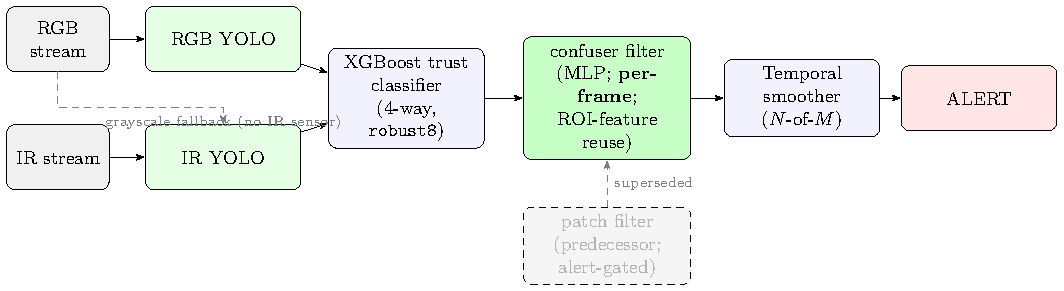
\includegraphics[width=\textwidth]{figures/fig_pipeline.pdf}
    \caption{Multi-stage drone detection pipeline. The production confuser verifier is the distilled \texttt{mlp\_v5}, which runs \textbf{per frame} because it reuses the detectors' already-computed ROI features rather than re-processing crops (\S\ref{sec:distill_verifier}). It supersedes the MobileNetV3 patch verifier (greyed), which was expensive enough that it had to be \emph{alert-gated} --- consulted only when the temporal smoother was about to fire (\S\ref{sec:alert_gate}).}
    \label{fig:pipeline}
\end{figure}

The downstream stages contribute the majority of confuser suppression without retraining the detectors. Three architectural choices make this possible: fail-open detection (\S\ref{sec:design_rationale}), trust-aware fusion (\S\ref{sec:trust_fusion}), and a downstream confuser verifier --- in production the per-frame distilled \texttt{mlp\_v5} (\S\ref{sec:distill_verifier}).

\paragraph{A note on the verifier across the evaluation chapters.} The production confuser verifier is the per-frame distilled \texttt{mlp\_v5} (RGB, \S\ref{sec:distill_verifier}) and its cross-modal counterpart \texttt{mlp\_v5\_ir\_aligned} (IR, \S\ref{sec:ir_xmodal_verifier}). The full-cascade experiments in Section~\ref{ch:experiments} were run with the older MobileNetV3 patch verifier at the alert gate; those numbers are therefore conservative relative to the production stack. A full-pipeline re-evaluation with \texttt{mlp\_v5} is a registered open item (\S\ref{sec:realvideo_cascade}); component-level evidence that \texttt{mlp\_v5} dominates the patch verifier on every confuser-rich surface is in \S\ref{sec:distill_verifier}.

\paragraph{Two-verifier fusion (trust-first).} With both RGB (\texttt{mlp\_v5}) and IR (\texttt{mlp\_v5\_ir\_aligned}) verifiers running per-frame, fusion is \emph{trust-first}: the trust classifier (\S\ref{sec:trust_fusion}) routes, then the trusted modality's verifier filters. \texttt{reject\_both} drops the frame; \texttt{trust\_rgb} keeps it only if the RGB verifier passes; \texttt{trust\_ir} keeps it only if the IR verifier passes; \texttt{trust\_both} is resolved per-modality (recall-first: the detection survives if either trusted verifier passes), with a cross-modal soft-weighted tie-break left as future work. The IR verifier can run always-on because the grayscale$\leftrightarrow$thermal alignment (\S\ref{sec:ir_xmodal_verifier}) makes it recall-safe rather than recall-eroding. This ordering is classifier-agnostic: it is unchanged whether the router is the shipped \texttt{robust8} (its \texttt{robust6} base, \S\ref{sec:feature_selection}) or the \texttt{sa32} comparison classifier.
% [source: ledger=dual-verifier-fusion-rule; run=eval/overnight_ablation.py; config=clf_own_holdout]

\subsection{Design Rationale: Fail-Open}
\label{sec:design_rationale}

The cascade's central design principle is asymmetric recoverability: a confuser false positive raised by the detector can be vetoed downstream, but a drone the detector missed cannot be recovered by any later stage. The cascade therefore ``fails open'' at the detector, deferring suppression rather than suppressing early at the cost of unrecoverable misses. Both detectors are trained with confuser negatives (\S\ref{sec:rgb_three_variants}, \S\ref{sec:ir_detector}), but training-time mining does not eliminate all categories: bird hallucination at the RGB detector is irreducible at small drone sizes (\S\ref{sec:lit_fusion}). The cascade is built around that residual: the downstream stages catch what training cannot, especially on bird-on-sky and OOD imagery.

The cost is real and is visible in the same evaluation as the win. The three RGB-detector variants (Table~\ref{tab:rgb_comparison}) trace the lever: the baseline reaches drone $R=0.961$ on Svanstr\"om with a 94.4\% bird-frame fire rate; \texttt{retrained\_v2} cuts bird-frame fire to 3.4\% but drops drone recall to $R=0.306$. The collapse is Svanstr\"om-specific (on Roboflow OOD drones the same \texttt{retrained\_v2} retains $R=0.726$ vs baseline $R=0.746$), but for any deployment that must catch small drones it is disqualifying.
% [source: ledger=retrainedv2-recall-collapse; eval=rgb_svan_retrainedv2,rob_rgb_retrainedv2,rob_rgb_baseline; run=eval/diagnose_failures_all.py; cache=eval/results/_failure_diagnosis/svanstrom_1280_by_category.csv; config=svan_iop_1280]

The cascade uses the downstream stages to reduce OOD confuser fire rate, at an in-distribution cost that is operating-point-dependent. On the OOD confuser zoo with \texttt{fusion\_no\_fn\_v1.1}, the classifier carries the bulk of the suppression ($52.1\% \to 1.6\%$) and the patch verifier roughly halves the residual ($1.6\% \to 0.8\%$). With \texttt{sa32} the suppression is shallower but still substantial ($52.1\% \to 20.5\% \to 10.3\%$). On Svanstr\"om paired drones the stages drop trust-aware $F1$ from 0.950 (S1) to 0.914 (S2) to 0.868 at \texttt{patch\_thr}$=$0.5, recovering to 0.895 at \texttt{patch\_thr}$=$0.9. On the real-video diagnostic (run with \texttt{sa32} and the predecessor patch verifier, $\mathtt{patch\_thr}=0.7$; the production \texttt{robust8}/\texttt{mlp\_v5} re-run is a registered open item, \S\ref{sec:realvideo_cascade}), temporal smoothing recovers per-frame misses and the full cascade lifts baseline-RGB drone segment $F1$ from $0.760$ to $0.826$ while cutting confuser segment FPR from $0.512$ to $0.162$ ($-68\%$) (\S\ref{sec:realvideo_cascade}). The exchange between in-distribution $F1$ and OOD safety is jointly driven by the classifier and the evaluation surface (RQ2; \S\ref{sec:rq_answers}), not by the cascade structure itself.
% [source: ledger=cascade-confuser-collapse; eval=clfzoo_fnfn; run=eval/cumulative_halluc.py; cache=eval/results/_cumulative_halluc/confuser_fusion_no_fn_model_v1.1/summary.json; config=confuser_zoo_1280]

\subsection{Trust-Aware Fusion}
\label{sec:trust_fusion}

The fusion stage is a learned per-frame decision rather than a fixed vote. The classifier outputs one of four labels:

\begin{itemize}
    \item \textbf{\texttt{reject\_both}}, neither modality's detection is trustworthy (likely a confuser).
    \item \textbf{\texttt{trust\_rgb}}, only RGB is reliable for this frame.
    \item \textbf{\texttt{trust\_ir}}, only IR is reliable for this frame.
    \item \textbf{\texttt{trust\_both}}, both modalities agree and are trustworthy.
\end{itemize}

The 4-way formulation captures \emph{when} each modality is reliable. The data-supported asymmetry is not primarily a lighting one: on Svanstr\"om paired data the IR detector ($P=0.950, R=0.973, F1=0.961$) is stronger than the RGB detector (drone $F1=0.950$, Table~\ref{tab:rgb_comparison}), and on the real-video diagnostic the IR detector fed grayscale-RGB sits on the Pareto frontier --- $3.2\times$ lower aggregate confuser FPPI ($0.158$ vs $0.512$) at $-12.4$~pp drone F1 (\S\ref{sec:realvideo}). The asymmetry the classifier exploits is that \emph{the two detectors hallucinate on different scenes}: visual confusers fool the RGB detector more reliably; thermally degraded conditions fool the IR detector more reliably. A per-frame classifier can pick the modality whose failure profile is least active; a fixed-weight rule cannot.
% [source: ledger=no-pareto-dominance-video; eval=vid_drone_ir_gray; run=eval/eval_video_tests.py; config=video_drone_iop]

The production stack uses the six free, leakage-aware features of \texttt{robust6} (\S\ref{sec:feature_selection}), which statistically supersede the 32-feature \texttt{sa32} that served as the working pick through the real-video comparison (\S\ref{sec:realvideo_classifier}). Two hand-engineered alternatives are retained: \texttt{control\_v3more\_40feat} for confuser-dense surfaces, and \texttt{fusion\_no\_fn\_v1.1} for open-world deployment (\S\ref{sec:classifier_variants}).
% [source: ledger=robust6-production-viable,ft4-lean-trust-classifier; run=classifier/train_lean_ft4.py; cache=docs/analysis/2026-05-31_ft4_lean_trust_classifier.md; config=clf_own_holdout] Detector signals (in particular the presence of an IR detection) are among the most informative features in every variant, but the exact ranking is variant-specific and is reported per classifier rather than asserted as a global ``IR detection contributes $X\%$'' figure.

\subsection{Alert-Gate Cascade}
\label{sec:alert_gate}

This section describes the MobileNetV3 \emph{patch} verifier, the predecessor that \texttt{mlp\_v5} (\S\ref{sec:distill_verifier}) supersedes. Alert-gating was forced by the patch verifier's cost (a second CNN over crop pixels) and is retained here because it is the design under which the patch verifier was audited.

The patch verifier is positioned at the \emph{alert gate}: it is consulted only when the temporal smoother is about to emit an alert (i.e., when the rolling per-frame decision window is about to complete an alert-triggering majority). Two alternative cascades were considered and rejected:

\begin{itemize}
    \item \textbf{\texttt{filter\_then\_classifier}}, run the patch verifier on every detection \emph{before} the trust classifier. Per-frame patch filtering cost $\approx 1$~pp Svanstr\"om F1 by vetoing marginal drone TPs whose patch probability fell into the soft middle of the verifier's distribution (\texttt{D\_cascade}).
    \item \textbf{\texttt{classifier\_then\_filter}}, run the patch verifier on every frame after the classifier accepts. Same problem at smaller magnitude.
\end{itemize}

Both are implemented in \texttt{eval/eval\_pipeline.py} but neither matches production. The production cascade is \texttt{alert\_gate\_only}, implemented in \texttt{eval/eval\_video\_temporal.py} and in the PySide GUI's \texttt{should\_suppress\_alert(\dots)} (\texttt{ir\_gui/pyside\_engine.py}). The verifier's CNN runs only at the moment a temporal window resolves into an alert, so the per-frame latency cost of the verifier is zero on the overwhelming majority of frames.

\subsection{Temporal Smoother}
\label{sec:temporal}

The temporal smoother is an $N$-of-$M$ sliding-window aggregator with configurable cooldown. An alert fires only when the trust classifier's per-frame decision has been positive on at least $N$ of the last $M$ frames, absorbing isolated firings characteristic of birds and aircraft transiting the field of view.

The same temporal state drives a \emph{ROI fallback} in the PySide engine (\texttt{\_run\_with\_roi}). When the full-frame YOLO returns nothing and a recent track is still alive, YOLO is re-run on an expanded crop around the previous box at reduced confidence. This is a GUI-only feature, and the frame-mode evaluation harness does not use it; it accounts for part of the GUI-versus-eval performance gap on small distant drones. The GUI maintains tracks and renders a path image, but does not yet classify on track-level features (flight dynamics); track-level classification is a promising direction for future work.

Frame-independent evaluation (the standard mode in \texttt{eval/cumulative\_halluc.py}) omits the temporal smoother so per-stage contributions can be measured cleanly; the reported metrics are therefore lower bounds on the deployed system's confuser rejection.

\begin{figure}[htbp]
    \centering
    \fbox{\parbox{0.9\textwidth}{\centering\vspace{2cm}
        \textbf{[PLACEHOLDER: Fig 3.2 --- PySide6 deployment GUI]} Annotated screenshot of the deployed GUI: dual-modality view (RGB + IR side by side), per-frame trust-label readout, sliding temporal window indicator, alert banner, ROI fallback crop inset, drone-path overlay across recent frames, threshold sliders for RGB / IR / patch.
    \vspace{2cm}}}
    \caption{PySide6 deployment GUI. The temporal smoother's state, the trust classifier's per-frame decision, and the ROI fallback crop are all surfaced for the human operator; the patch verifier runs silently at the alert gate.}
    \label{fig:pyside_gui}
\end{figure}

\subsection{Resolution Dependency}
\label{sec:resolution_arch}

Resolution is the single largest hyperparameter affecting small-drone recall. Svanstr\"om's native resolution is $640\times 512$; at \texttt{imgsz=1280} the baseline RGB detector reaches $R=0.961$ on Svanstr\"om drones, whereas at \texttt{imgsz=640} small drones fall below the resolvable floor (\texttt{retrained\_v2} collapses to $R=0.072$ at that size). Anti-UAV imagery ($1920\times 1080$) saturates at \texttt{imgsz=640} because drones already span enough pixels. All Svanstr\"om RGB evaluation uses \texttt{imgsz=1280}. SelCom CCTV is a third regime: clutter is the binding constraint, and the imgsz sweep in \texttt{docs/analysis/2026-05-16\_rgb\_camera\_spec\_and\_fault\_profile.md} identifies $\mathtt{imgsz}=960$ as the F1-optimal setting for that camera.
% [source: ledger=selcom-imgsz-win; eval=rgb_svan_baseline; run=eval/diagnose_failures.py; cache=eval/results/_failure_diagnosis/svanstrom_1280_by_category.csv; config=svan_iop_1280]

\begin{figure}[htbp]
    \centering
    
\includegraphics[width=0.85\textwidth]{fig6_6_resolution}
    \caption{Inference-resolution dependency of Svanstr\"om drone recall. At \texttt{imgsz=1280} the baseline detector reaches $R=0.961$; the \texttt{imgsz=640} floor is illustrated with \texttt{retrained\_v2} ($R=0.072$), the only variant measured at that size --- the baseline's own \texttt{imgsz=640} run is pending (\S\ref{sec:resolution_arch}), so the two endpoints are different variants and the curve is indicative, not a single-model sweep.}
    % [source: ledger=retrainedv2-recall-collapse; eval=rgb_svan_baseline; run=eval/diagnose_failures.py; cache=eval/results/_failure_diagnosis/svanstrom_1280_by_category.csv; config=svan_iop_1280]
    \label{fig:resolution}
\end{figure}

\subsection{RGB Drone Detector}
\label{sec:rgb_detector}

The RGB detector is a YOLOv26n (nano) single-class detector trained on Anti-UAV RGB frames~\cite{jiang2021antiuav}, Roboflow community drone datasets, and a drone-vs-bird subset as deliberate confuser negatives. Svanstr\"om imagery is held out from training. The three variants below explore how much additional confuser-specific data to add on top of this baseline corpus.

\subsubsection{Three Training Stances}
\label{sec:rgb_three_variants}

Three RGB-detector variants were trained and compared, representing three operating points on the recall--hallucination axis.

\begin{enumerate}
    \item \textbf{Baseline} (\texttt{Yolo26n\_trained}). Trained on the composite drone corpus, which includes the drone-vs-bird subset as deliberate confuser negatives but does not include Svanstr\"om-style confuser splits as explicit negatives. On Svanstr\"om@1280 it reaches $P=0.940, R=0.961$ on drones.
    % [source: ledger=retrainedv2-recall-collapse; eval=rgb_svan_baseline; run=eval/diagnose_failures.py; cache=eval/results/_failure_diagnosis/svanstrom_1280_by_category.csv; config=svan_iop_1280]
    \item \textbf{\texttt{hardneg\_v3more}} (\texttt{Yolo26n\_hardneg\_v3more}). Same backbone, retrained with the Svanstr\"om bird/airplane/helicopter confuser splits supplied as additional negatives. Drone $P=0.941, R=0.950$; helicopter fire rate drops from 66.2\% to 41.9\%, airplane fire rate from 74.6\% to 64.7\%, but bird fire rate is essentially unchanged at 94.2\%.
    % [source: ledger=retrainedv2-recall-collapse; eval=rgb_svan_baseline; run=eval/diagnose_failures.py; cache=eval/results/_failure_diagnosis/svanstrom_1280_by_category.csv; config=svan_iop_1280]
    \item \textbf{\texttt{retrained\_v2}} (\texttt{Yolo26n\_retrained\_v2}). Aggressive retraining with heavy confuser augmentation. Bird fire rate collapses to 3.4\% but Svanstr\"om drone recall collapses to $R=0.306$ at the same operating threshold. The collapse is Svanstr\"om-specific: on Roboflow OOD drone splits the same weights retain $R=0.726$.
    % [source: ledger=selcom-ood-confuser-damage; eval=rob_rgb_retrainedv2; run=eval/run_roboflow_eval.py; config=roboflow_rgb_drone_640]
\end{enumerate}

The improvement is class-specific: adding Svanstr\"om confuser negatives works for helicopters, partially for airplanes, and not for birds (no change). Birds and small drones share too much low-level structure for the YOLO feature extractor to discriminate reliably without an unacceptable recall cost. The cascade targets specifically the bird case; helicopter and airplane suppression is achievable at the detector stage, as the \texttt{hardneg\_v3more} row shows.

\begin{table}[htbp]
    \centering
    \caption{RGB variants on Svanstr\"om @ \texttt{imgsz=1280} (IoP@0.5, drone class). Aggressive retraining destroys recall on small Svanstr\"om drones while leaving Roboflow OOD performance comparable.}
    \label{tab:rgb_comparison}
    \begin{tabular}{lccccc}
        \toprule
        Model & Drone $P$ & Drone $R$ & Bird halluc & Airplane halluc & Heli halluc \\
        \midrule
        baseline           & 0.940 & \textbf{0.961} & 94.4\% & 74.6\% & 66.2\% \\
        \texttt{hardneg\_v3more}  & 0.941 & 0.950 & 94.2\% & 64.7\% & 41.9\% \\
        \texttt{retrained\_v2}    & 0.943 & 0.306 & \textbf{3.4\%}  & \textbf{5.6\%}  & \textbf{4.5\%}  \\
        \bottomrule
    \end{tabular}
\end{table}

The same comparison at \texttt{imgsz=640} on Svanstr\"om was run for \texttt{retrained\_v2} ($P=0.837, R=0.072$) and confirms that the \texttt{imgsz=640} regime is unusable for Svanstr\"om regardless of variant; the equivalent \texttt{imgsz=640} runs for the baseline and \texttt{hardneg\_v3more} are flagged as TBD (placeholder).
% [source: ledger=retrainedv2-recall-collapse; eval=rgb_svan_baseline; run=eval/diagnose_failures.py; cache=eval/results/_failure_diagnosis/svanstrom_1280_by_category.csv; config=svan_iop_1280]

\subsubsection{SelCom CCTV Fine-Tune}
\label{sec:selcom_finetune}

A separate fine-tune line targets a fixed-camera 7~Mbps HEVC CCTV stream from deployment partner SelCom. The fine-tune is on top of the \emph{baseline} \texttt{Yolo26n\_trained} weights (not \texttt{retrained\_v2}), keeping the cascade compatible with the deployed classifier without a recalibration swap. Selcom drones are small (median $\sqrt{\text{area}} \approx 37$~px in the source frame) and blend into urban clutter. Two mixed-training fine-tunes (80\% general RGB + 20\% selcom; pure-selcom val split, seed 0) were evaluated at IoP@0.5, conf$=$0.25 on \texttt{selcom\_mixed\_ft2\_val} (311 images, 295 GT boxes):
% [source: ledger=selcom-imgsz-win; eval=selcom_ft2_1280; run=RGB model/finetune_selcom.py; cache=runs/rgb_finetune_eval/Yolo26n_selcom_mixed_ft2_1280/comparison.json; config=selcom_iop_1280]

\begin{table}[htbp]
    \centering
    \caption{SelCom CCTV fine-tune; IoP@0.5, conf=0.25, val split 311~imgs / 295~GT. The production CCTV stack uses \texttt{Yolo26n\_selcom\_mixed\_ft2\_1280}.}
    \label{tab:selcom}
    \begin{tabular}{lcccccc}
        \toprule
        Model & imgsz & TP & FP & FN & $P$ & $R$ \\
        \midrule
        baseline (\texttt{Yolo26n\_trained})        & 640  &   2 &  6 & 293 & 0.250 & 0.007 \\
        baseline                                    & 1280 &  26 & 37 & 269 & 0.413 & 0.088 \\
        \texttt{Yolo26n\_selcom\_mixed\_ft2}        & 640  &  72 & 50 & 223 & 0.590 & 0.244 \\
        \textbf{\texttt{Yolo26n\_selcom\_mixed\_ft2\_1280}} & \textbf{1280} & \textbf{138} & \textbf{43} & \textbf{157} & \textbf{0.762} & \textbf{0.468} \\
        \bottomrule
    \end{tabular}
\end{table}

The \texttt{ft2\_1280} weights double selcom recall vs \texttt{ft2@640} (0.244 $\to$ 0.468) while raising precision (0.590 $\to$ 0.762). The regression on the standard RGB dataset is within $-0.008$ F1 of baseline. A preprocessing sweep established that no OpenCV variant (denoise, CLAHE, sharpen, contrast) improves detection independently of fine-tuning and \texttt{imgsz}; the relevant levers are training data and resolution.
% [source: ledger=selcom-imgsz-win; eval=selcom_ft2_1280; run=RGB model/finetune_selcom.py; cache=runs/rgb_finetune_eval/Yolo26n_selcom_mixed_ft2_1280/comparison.json; config=selcom_iop_1280]

The imgsz sweep on selcom (4~models $\times$ 4~sizes $\times$ 3~datasets) points to $\mathtt{imgsz}=960$ as the F1-optimal CCTV setting. Above that, clutter-driven FPs grow faster than drone recall improves.

\subsection{IR Drone Detector}
\label{sec:ir_detector}

The IR detector uses the same YOLOv26n architecture finetuned on iteratively curated thermal data (\S\ref{sec:hitl_ir}). Bird, airplane, and helicopter thermal frames are added as hard negatives across HITL revisions. The production weights (\texttt{v3b}) are a 2-epoch corrective fine-tune on the \texttt{Final} checkpoint addressing specific deployment-time failure modes. The full evolution across six numbered revisions --- including the V5 regression and its recovery --- is in Chapter~\ref{ch:hitl} (\S\ref{sec:ir_evolution}).

\subsubsection{IR Detector on Svanstr\"om and Anti-UAV}

Under the May~10 ablation matrix, IR-only on Svanstr\"om at \texttt{imgsz=640} reaches $P=0.950, R=0.973, \text{F1}=0.961$ (TP$=$2234, FP$=$117, FN$=$63); on Anti-UAV it reaches $P=0.987, R=0.945, \text{F1}=0.9654$. The IR detector is the stronger single-modality detector on both benchmarks. The trust classifier therefore chooses between two competent modalities with different failure profiles, not between a weak and a strong one. The IR detector's brittleness is on OOD thermal imagery ($R=0.519$ on \texttt{ir\_mixed\_cbam}, $R=0.264$ on \texttt{ir\_drone\_night}; \S\ref{sec:roboflow}), which is what motivates retaining the RGB detector.
% [source: ledger=prov-may10-imgsz; eval=ir_v3b_svan640_may10; run=(May-10 ablation matrix); cache=eval/results/_ablation/2026-05-10T16-08-14/master.csv; config=svan_iop_640_may10]

\subsubsection{Grayscale-RGB Operating Mode}
\label{sec:ir_grayscale_mode}

The deployed PySide GUI exposes a \emph{grayscale-RGB} operating mode (\texttt{\_infer\_grayscale}). When no thermal camera is available, the GUI converts the RGB stream to grayscale via \texttt{cvtColor(BGR2GRAY)}, replicates to three channels, and feeds the result to the IR detector at \texttt{imgsz=640}. On the real-video diagnostic this fallback sits on the Pareto frontier. It ties the RGB baseline on the hardest bird-cluttered clip, despite having never seen visible-light data in training. Full quantification and limits are in \S\ref{sec:grayscale}. The design point: on some scenes the fallback is on par with the best visible-light detector, not a strict degradation mode.

\subsubsection{Cross-Modal Feature Alignment: a Thermal Verifier from Grayscale Confusers}
\label{sec:ir_xmodal_verifier}

The same grayscale-RGB mode dissolves the data-scarcity blocker that had previously kept any per-frame IR confuser verifier out of the production stack. The argument has two feature-space steps, both measured with the Model MRI tool (\S\ref{sec:model_mri}).

\emph{First, the confuser-rejection signal already lives inside the IR detector.} An MRI of the \texttt{v3b} fused \texttt{p3}+\texttt{p5} ROI features (517-D), over $14{,}697$ drone and $1{,}386$ confuser detections mined across IR surfaces, shows the two classes are almost linearly separable. A single linear discriminant reaches $0.981$ train accuracy, and the strongest single neuron --- a \texttt{p5} channel --- carries an ANOVA $F=5{,}370$, a near-binary ``is-this-a-drone'' switch against a raw detector hallucination rate of only $1.8\%$/image. A linear probe projects an $89\%$ false-positive cut at a $10\%$ recall cost. The signal is spatial rather than confidence-based: ranked by per-class z-score the top discriminators are \texttt{p5} semantic channels, while the detection-confidence scalar (\texttt{meta:conf}) ranks far down. Rendering the activations on real detections reproduces the RGB verifier's signature (the thermal counterpart of Figure~\ref{fig:mri_activation}). On a thermal drone the \texttt{p3} activation binds to the airframe and \texttt{p5} forms a centred semantic blob; on a held-out CBAM confuser false-fire the same neurons scatter across background. The IR feature space is, in short, the thermal twin of the RGB verifier's (\S\ref{sec:distill_verifier}, Figure~\ref{fig:mri_stats}): the same near-linear separability, readable by the same kind of lightweight MLP with no detector retraining.
% [source: ledger=ir-features-separable; eval=none (MRI run); run=mri/cli.py; cache=mri/results/ir_v3b_report; config=ir_v3b]

\emph{Second, the grayscale$\rightarrow$thermal feature gap is a removable affine offset, so a confuser filter transfers across the modality.} The detector represents a given class almost identically in real thermal and in grayscale-RGB: the top-discriminative neurons overlap (Jaccard $0.71$--$0.88$), the mean-activation signatures correlate at $0.93$--$0.99$, and the drone-class centroids sit at cosine distance $0.012$. The only systematic difference is a per-feature mean/scale offset. Removing it with a \emph{per-modality z-score} (\S\ref{sec:model_mri}) lifts grayscale$\rightarrow$thermal confuser-transfer AUROC from $0.500$ (chance, no alignment) to $0.919$, against a within-thermal cross-validated ceiling of $0.974$; full-covariance CORAL reaches only $0.707$, which confirms the gap is a diagonal mean/scale shift rather than a representational change (Figure~\ref{fig:ir_gray_align}).
% [source: ledger=gray-thermal-alignable; eval=none (MRI modality probe); run=mri/modality_align.py; cache=mri/results/ir_v3b_report; config=ir_v3b]

\begin{figure}[htbp]
    \centering
    
\includegraphics[width=\textwidth]{fig9_ir_gray_align}
    \caption{Grayscale$\leftrightarrow$thermal feature alignment in the IR detector. (A) After a per-modality z-score, thermal and grayscale drones land in the same region of the drone-vs-confuser discriminant axis, and likewise for confusers --- the modalities are interchangeable up to an affine offset. (B) Grayscale-trained confuser-filter transfer to thermal rises from chance ($0.500$) to near the within-thermal ceiling ($0.919$ vs $0.974$) once the offset is removed; CORAL ($0.707$) under-performs the simpler z-score.}
    % [source: ledger=gray-thermal-alignable; eval=none (MRI modality probe); run=mri/modality_align.py; cache=mri/results/ir_v3b_report; config=ir_v3b]
    \label{fig:ir_gray_align}
\end{figure}

Together these show that the IR confuser-verifier blocker was data scarcity, not the detector: labelled thermal confusers are rare, but grayscale-RGB confusers are abundant and, once z-aligned, occupy the same thermal feature space. Harvesting them yields a thermal verifier that is both confuser-rich and recall-safe. The deployed checkpoint and its held-out evaluation --- which reverse the earlier ``ship no IR verifier'' conclusion --- are reported in \S\ref{sec:grayscale_verifier}.
% [source: ledger=ir-grayscale-harvest-solves-thermal-verifier; eval=ir_aligned_cbam_heldout; run=mri_train_aligned; config=cbam_ir_640]

\subsection{Trust Classifier}
\label{sec:trust_classifier}

\subsubsection{Feature Set}

The trust classifier consumes per-frame features from the two detectors' raw outputs and the source frames. The shipped classifier is the six-feature \texttt{robust6} (\S\ref{sec:feature_selection}); the hand-engineered comparison set is \texttt{sa32} (32 features) and the two 40-feature variants \texttt{control\_v3more\_40feat} and \texttt{fusion\_no\_fn\_v1.1}. The feature families are common across the larger variants:
% [source: ledger=ft4-lean-trust-classifier; run=classifier/train_lean_ft4.py; config=clf_own_holdout]

\begin{itemize}
    \item \textbf{Detector signals}: per-modality binary detection flags, top-$k$ confidence scores, detection counts.
    \item \textbf{Scene features}: image intensity statistics, edge density, frequency-domain summaries; intended to detect ``confuser-rich'' scenes vs ``clean sky'' scenes.
    \item \textbf{Target features}: bounding-box geometry (aspect ratio, normalised area, position), confidence distribution per modality.
    \item \textbf{Agreement features}: cross-modal IoU, centre distance, confidence ratio.
    \item \textbf{Failure-model scores} (only in \texttt{control\_v3more\_40feat}): scalar outputs from a small per-modality failure-prediction network. \texttt{fusion\_no\_fn\_v1.1} explicitly drops these because they over-fitted to training-set artefacts and degraded OOD behaviour (see \S\ref{sec:classifier_variants}).
\end{itemize}

The label space is the 4-way trust decision of \S\ref{sec:trust_fusion}. The model is an XGBoost~\cite{chen2016xgboost} gradient-boosted classifier. Training uses sequence-stratified group shuffling so that frames from a given Anti-UAV or Svanstr\"om sequence are not split across train and test; this avoids the easy-leakage variant of cross-validation common in video classification.

The Svanstr\"om frames used to train the classifier overlap with those used to evaluate the full cascade in Section~\ref{ch:experiments}; this is flagged as a threat to validity (\S\ref{sec:threats}) and partially mitigated by the uncontaminated Anti-UAV results. Classifier behaviour across the three surfaces is quantified in \S\ref{sec:classifier_compare} and Section~\ref{ch:experiments} (\S\S\ref{sec:cumulative}, \ref{sec:realvideo_classifier}).

\subsubsection{Classifier Variants}
\label{sec:classifier_variants}

Three hand-engineered classifier variants form the comparison set. They share the same labelled paired-frame data and differ in feature engineering and OOD resilience. The strongest is \texttt{sa32} (the working pick through the real-video comparison, \S\ref{sec:realvideo_classifier}), with \texttt{fusion\_no\_fn\_v1.1} as the open-world fallback and \texttt{control\_v3more\_40feat} deprecated. The shipped \texttt{robust6} (\S\ref{sec:feature_selection}) is derived statistically and is the reference the variants below serve to bound.
% [source: ledger=ft4-lean-trust-classifier,robust6-production-viable,fusion-feature-leakage; run=classifier/train_lean_ft4.py; cache=docs/analysis/2026-05-31_ft4_lean_trust_classifier.md; config=clf_own_holdout]

\begin{itemize}
    \item \textbf{\texttt{scene\_aware\_v3more\_32feat} (\texttt{sa32}; strongest hand-engineered variant, superseded by \texttt{robust6})}: 32-feature variant with the failure-model scores dropped. Wins on the real-video diagnostic by 18--22 pp drone segment $F1$ over \texttt{control\_v3more\_40feat} and by 60+ pp over \texttt{fusion\_no\_fn\_v1.1} (\S\ref{sec:realvideo_classifier}). Ties \texttt{control\_v3more\_40feat} on Svanstr\"om within 1.3 pp drone $F1$ and ties it on the OOD confuser zoo (S2 fire 0.205 vs 0.212; S3 fire 0.103 vs 0.094). Higher OOD-zoo fire rate than \texttt{fusion\_no\_fn\_v1.1}, which is the operational cost of its drone-recall preservation.
    % [source: ledger=three-classifier-realvideo; eval=pipe3clf_sa32; run=(EVIDENCE_LEDGER sweep); config=pipe_video_drone_iop]
    \item \textbf{\texttt{fusion\_no\_fn\_v1.1} (open-world fallback)}: 40-feature variant trained with the failure-model scores explicitly dropped, sourced from the legacy fusion training pipeline. Substantially more conservative on OOD imagery ($\sim$1.6\% S2 zoo fire rate vs 20.5\% for sa32, a 13$\times$ reduction), but rejects 85\% of correct RGB drone TPs on the real-video diagnostic (\S\ref{sec:realvideo_classifier}, segment-level drone $R$ collapses to $0.128$ for baseline RGB). The right choice when missed drones cost less than confuser-induced false alarms; the wrong choice for general-purpose alert deployment.
    % [source: ledger=cascade-confuser-collapse; eval=pipe3clf_fnfn; run=(EVIDENCE_LEDGER sweep); config=pipe_video_drone_iop]
    \item \textbf{\texttt{control\_v3more\_40feat} (deprecated)}: 40-feature variant with failure-model scores retained. Equivalent to sa32 on Svanstr\"om and on the OOD confuser zoo within rounding, but loses 18--22 pp drone segment $F1$ on the real-video diagnostic. No operational regime favours it over sa32 on the joint axis; it was a production candidate prior to the real-video classifier comparison and is retained in the comparison tables for completeness.
\end{itemize}

The early \texttt{retrained\_v2\_32feat} classifier is superseded because the production RGB detector is no longer \texttt{retrained\_v2}; a training-time/production confidence-distribution mismatch accounts for most of the gap in comparison results. A trust classifier is not portable across RGB detector swaps without re-checking calibration.

\paragraph{Scene-fingerprint over-fitting.}
Under sequence-stratified splitting, per-clip image statistics act as \emph{scene fingerprints}: the classifier learns which clip a frame came from rather than whether a drone is present, inflating in-distribution scores while degrading transfer. Dropping these features (the \texttt{lean13}$\to$\texttt{lean10} pruning) recovers $18$--$26$~pp drone $F1$ on held-out clips; \texttt{sa32} already omits them by design. \S\ref{sec:feature_selection} turns this hindsight observation into a statistic computed before training.
% [source: ledger=scene-fingerprint-overfit; eval=own_lean10_yt,own_lean13_yt; run=(classifier feature-selection ablation); config=clf_own_holdout]

\paragraph{A dual-classifier extension for the missing-modality regime.}
A single classifier must serve both the paired RGB+IR regime and the grayscale-only fallback, whose feature distributions differ. Splitting it into a \emph{dual} architecture --- a 24-feature paired model and a separate 32-feature grayscale model --- strictly dominates single \texttt{sa32} on the missing-modality cases: on the RGB-fallback bird-confuser the drone $F1$ rises $0.247\to1.000$, on the \texttt{drone\_seagull} clip $0.461\to0.942$, and on \texttt{rgb\_dataset\_test} $0.690\to0.960$, while the paired-core performance is unchanged. The grayscale-fallback airplane and helicopter cases remain weak ($F1\approx0.50$, pending further hard-negative mining), so the dual classifier is reported as a validated extension rather than the shipped default.
% [source: ledger=dual-classifier-v3; eval=dualclf_v3_vs_sa32; run=(EVIDENCE_LEDGER sweep); config=dual_clf_v3_surfaces]

\paragraph{A grayscale-fallback recall hole in \texttt{robust6}.}
The \texttt{robust6} classifier (\S\ref{sec:feature_selection}; the base for the shipped \texttt{robust8}) inherits one honest weakness from its lean feature set. In the grayscale-RGB fallback regime (no thermal sensor), all three of \texttt{robust6}'s IR features and the cross-modal ratio go to chance (single-feature AUROC $\approx 0.51$) because the IR inputs are dead, leaving only the RGB features and \texttt{conf\_sum} live. The consequence is a \texttt{trust\_rgb} \emph{recall} failure: drone-only-in-RGB frames are routed to \texttt{reject}, and grayscale drone recall collapses to $R\approx0.19$, while \texttt{trust\_both} ($F1\approx0.98$) and thermal \texttt{trust\_ir} ($\approx0.92$) remain healthy. The first reading was that this needs an architectural fix (regime-aware routing); \S\ref{sec:feature_selection} shows instead that two free features (\texttt{rgb\_mean\_conf} and an \texttt{is\_grayscale} flag) and a per-class \texttt{trust\_rgb} threshold close it --- the \texttt{robust8} extension --- recovering grayscale recall at a measured real-video-confuser cost.
% [source: ledger=robust6-grayscale-ir-features-dead,routing-failure-is-trust-rgb-recall; run=classifier/train_lean_ft4.py; config=clf_own_holdout]

\subsubsection{Classifier Performance Comparison}
\label{sec:classifier_compare}

Three classifier variants were compared on Svanstr\"om (stride 9, IoP@0.5, baseline RGB, v2 patch verifier, \texttt{imgsz=1280}) and the OOD confuser zoo:

\begin{table}[htbp]
    \centering
    \caption{Classifier comparison. The split verdict between Svanstr\"om and the OOD zoo motivates the open-world vs calibrated-deployment distinction.}
    \label{tab:classifiers}
    \begin{tabular}{lccccccc}
        \toprule
        Classifier & thr & Drone S2 $R$ & Drone S2 F1 & Drone S3 $R$ & Drone S3 F1 & Zoo S2 & Zoo S3 \\
        \midrule
        \texttt{fusion\_no\_fn\_v1.1}        & 0.8/0.9 & 0.909 & 0.912 & 0.856/0.869 & 0.889/0.895 & \textbf{0.016} & \textbf{0.008} \\
        \textbf{\texttt{scene\_aware\_v3more\_32feat}} & 0.8 & 0.922 & 0.919 & 0.868 & 0.896 & 0.205 & 0.103 \\
        \texttt{control\_v3more\_40feat} & 0.9 & \textbf{0.934} & \textbf{0.925} & \textbf{0.893} & \textbf{0.909} & 0.212 & 0.094 \\
        \bottomrule
    \end{tabular}
\end{table}

\begin{figure}[htbp]
    \centering
    
\includegraphics[width=0.85\textwidth]{fig7_1_ood_classifier}
    \caption{Classifier comparison on the OOD confuser zoo. \texttt{fusion\_no\_fn\_v1.1} fires on $\sim$13$\times$ fewer frames than the comparison classifier \texttt{sa32} and the deprecated \texttt{control\_v3more\_40feat}; sa32 and control40 are tied within rounding on this benchmark. Source: \texttt{eval/results/\_cumulative\_halluc/confuser\_c40/summary.json}.}
    \label{fig:ood_classifier}
\end{figure}

\emph{Svanstr\"om.} \texttt{control\_v3more\_40feat} wins on every Svanstr\"om drone metric ($+2.5$~pp Stage-3 recall vs \texttt{scene\_aware}; $+1.3$~pp Stage-3 F1); within 1.3 pp the three are operationally indistinguishable.

\emph{OOD confuser zoo.} \texttt{fusion\_no\_fn\_v1.1} is $13\times$ more conservative than \texttt{scene\_aware} ($1.6\%$ vs $20.5\%$ S2 fire). \texttt{control\_v3more\_40feat} ties \texttt{scene\_aware} ($0.212$ vs $0.205$ S2; $0.094$ vs $0.103$ S3): the fnfn-vs-sa32 gap is load-bearing; the control40-vs-sa32 gap is not.
% [source: ledger=cascade-confuser-collapse; eval=clfzoo_fnfn; run=eval/cumulative_halluc.py; cache=eval/results/_cumulative_halluc/confuser_fusion_no_fn_model_v1.1/summary.json; config=confuser_zoo_1280]

\emph{Real video} (\S\ref{sec:realvideo_cascade}). \texttt{scene\_aware} dominates: cascade drone segment $F1$ = 0.826 baseline RGB, vs 0.644 for \texttt{control\_v3more\_40feat} ($-18$~pp) and 0.219 for \texttt{fusion\_no\_fn\_v1.1} ($-61$~pp). The Svanstr\"om-only ordering reverses on real-video; the Svanstr\"om benchmark does not by itself select the production classifier.
% [source: ledger=three-classifier-realvideo; eval=pipe3clf_sa32; run=(EVIDENCE_LEDGER sweep); config=pipe_video_drone_iop]

\paragraph{Deployment implication.}
Among the hand-engineered variants, \texttt{sa32} is the strongest: it ties or wins on every surface except a 1.3-pp gap on Svanstr\"om S3 F1 and strictly dominates on the real-video diagnostic. \texttt{control\_v3more\_40feat} buys nothing on the zoo and loses on real-video; it is deprecated. \texttt{fusion\_no\_fn\_v1.1} remains the open-world fallback where missed drones are operationally tolerable. \S\ref{sec:feature_selection} shows the six-feature \texttt{robust6} matches \texttt{sa32}'s in-domain accuracy while improving OOD robustness; its grayscale-hardened extension \texttt{robust8} is the shipped classifier.
% [source: ledger=robust6-production-viable; run=eval/overnight_ablation.py; cache=eval/results/_overnight_ablation/ablation_results.json; config=clf_own_holdout]

\subsubsection{Statistical Feature Selection: a Six-Feature Classifier}
\label{sec:feature_selection}

The variants above were assembled by hand; this subsection replaces that procedure with a statistical one. The motivating question is whether a measurable property can identify in advance which features carry the drone-versus-confuser signal and which only memorise scenes. Two practical pressures sharpen it: \texttt{sa32} was trained on detections from the superseded \texttt{selcom\_1280} detector (inputs no longer matching the production \texttt{ft4}/\texttt{v3b} detectors), and several of its features require an expensive per-frame OpenCV pass.
% [source: ledger=fusion-feature-leakage; run=classifier/fusion_feature_stats.py; cache=classifier/fusion_models/optimal_v1/feature_stats_ranked.csv; config=clf_own_holdout]

\paragraph{Method.}
From a cached $56$-feature matrix of $65{,}192$ frames we ran four analyses. LDA asks whether the signal is present: a single Fisher axis separates trust-positive from reject at $98.2\%$ training accuracy (Figure~\ref{fig:fusion_lda}), so the problem is \emph{selecting} features, not a signal shortage. PCA asks whether the structure is trivial: classes overlap in the top components, meaning scene-to-scene variance (brightness, texture) dominates over the drone signal --- the first indication that scene-statistic features dominate variance without carrying class signal. A per-feature ANOVA $F$-test and single-feature AUROC then rank each feature individually (Figure~\ref{fig:fusion_auroc}).
% [source: ledger=fusion-feature-leakage; run=classifier/fusion_feature_stats.py; cache=classifier/fusion_models/optimal_v1/feature_stats_ranked.csv; config=clf_own_holdout]

\paragraph{A leakage statistic.}
A scene-fingerprint feature can score as discriminative in a single pool simply because it correlates with which scene a sample came from; ANOVA and AUROC would recommend keeping it. To expose this we compute a second $F$-statistic \emph{within the drone class only} and form the ratio
\begin{equation}
\mathit{leakage\_ratio} = \frac{F_\text{domain-in-class}}{F_\text{class}},
\label{eq:leakage}
\end{equation}
which is low for a robust signal feature and high for a scene fingerprint. Equation~\ref{eq:leakage} converts the earlier hand-tuned deprecations into a number computed before any training run, measuring domain-dependence in order to discard it.
% [source: ledger=fusion-feature-leakage; run=classifier/fusion_feature_stats.py; cache=classifier/fusion_models/optimal_v1/feature_stats_ranked.csv; config=clf_own_holdout]

\begin{figure}[htbp]
    \centering
    \begin{subfigure}{0.32\textwidth}
\includegraphics[width=\textwidth]{fig8_fusion_lda}\caption{}\label{fig:fusion_lda}\end{subfigure}
    \hfill
    \begin{subfigure}{0.32\textwidth}
\includegraphics[width=\textwidth]{fig8_fusion_auroc}\caption{}\label{fig:fusion_auroc}\end{subfigure}
    \hfill
    \begin{subfigure}{0.32\textwidth}
\includegraphics[width=\textwidth]{fig8_fusion_leakage}\caption{}\label{fig:fusion_leakage}\end{subfigure}
    \caption{Statistical anatomy of the $56$-feature fusion space. (a) Linear discriminant: the trust signal is linearly separable ($98.2\%$ train accuracy). (b) Per-feature single-feature AUROC. (c) Leakage map (Eq.~\ref{eq:leakage}): the lower-right region is robust signal (high AUROC, near-zero leakage); the upper-left is scene fingerprint (chance-level AUROC, leakage in the hundreds). Source: \texttt{classifier/fusion\_feature\_stats.py}.}
    % [source: ledger=fusion-feature-leakage; run=classifier/fusion_feature_stats.py; cache=classifier/fusion_models/optimal_v1/feature_stats_ranked.csv; config=clf_own_holdout]
    \label{fig:fusion_stats}
\end{figure}

\paragraph{What the statistic finds.}
The leakage map separates two groups cleanly (Table~\ref{tab:leakage}). Scene-statistic features score at chance on the class label yet have leakage ratios in the hundreds --- they discriminate \emph{which scene}, not whether a drone is present, and are also the expensive per-frame features. The robust core --- detection confidences, box geometry, and cross-modal ratios --- scores AUROC above $0.9$ with leakage below $0.006$. A within-source check catches what the leakage ratio misses: \texttt{rgb\_blurriness} scores AUROC $0.872$ in the pooled set but collapses to $0.516$ within each source (a cross-clip mean-shift artefact), so the gate drops it alongside the scene fingerprints. Two caveats. Per-modality detection-presence flags top the AUROC chart but are excluded by reasoning, since the trust label is \emph{derived from} those detections. And the corpus is IR-dominant, so IR features rank above their RGB counterparts on RGB-fallback surfaces.
% [source: ledger=fusion-feature-leakage,blurriness-is-corpus-artifact; run=classifier/fusion_feature_stats.py,classifier/vet_blurriness_stats.py; cache=classifier/fusion_models/optimal_v1/feature_stats_ranked.csv; config=clf_own_holdout]

\begin{table}[htbp]
    \centering
    \caption{Leakage analysis splits the feature space. \emph{Top}: scene fingerprints --- chance-level class AUROC but very high leakage; drop. \emph{Bottom}: the robust core --- high AUROC, near-zero leakage; keep. Source: \texttt{feature\_stats\_ranked.csv}.}
    \label{tab:leakage}
    \begin{tabular}{llcc}
        \toprule
        feature & family & AUROC-alone & leakage ratio \\
        \midrule
        \multicolumn{4}{l}{\emph{Scene fingerprints (drop)}} \\
        \texttt{rgb\_img\_std}       & scene       & 0.502 & 349.6 \\
        \texttt{rgb\_img\_entropy}   & scene       & 0.510 & 307.4 \\
        \texttt{ir\_blurriness}      & scene       & 0.795 & 11.7 \\
        \texttt{rgb\_edge\_density}  & scene       & 0.525 & 1.75 \\
        \midrule
        \multicolumn{4}{l}{\emph{Robust core (keep)}} \\
        \texttt{conf\_sum}             & confidence  & 0.983 & 0.002 \\
        \texttt{ir\_max\_conf}         & confidence  & 0.965 & 0.002 \\
        \texttt{ir\_best\_aspect\_ratio} & geometry  & 0.952 & 0.002 \\
        \texttt{ir\_best\_log\_bbox\_area} & geometry & 0.946 & 0.005 \\
        \texttt{xmodal\_conf\_ratio}   & cross-modal & 0.905 & 0.002 \\
        \bottomrule
    \end{tabular}
\end{table}

\paragraph{The robust6 classifier.}
Applying the keep rule yields \texttt{robust6} $=$ \{\texttt{rgb\_max\_conf}, \texttt{ir\_max\_conf}, \texttt{rgb\_best\_log\_bbox\_area}, \texttt{ir\_best\_log\_bbox\_area}, \texttt{rgb\_best\_aspect\_ratio}, \texttt{ir\_best\_aspect\_ratio}\}: all free detector outputs and box geometry, all near-zero leakage. Training data is re-mined from the current \texttt{ft4}/\texttt{v3b} detectors, fixing the drift in \texttt{sa32}'s inputs. Two ablation levels confirm the design: in-domain $F1$ is flat as the feature count grows from $6$ to $32$ (count is not the lever), but on OOD drone video the set \emph{with} fingerprint features collapses to $F1=0.262$, climbing to $0.436$ then $0.578$ for \texttt{robust6} --- dropping fingerprints roughly doubles OOD generalisation. Dropping IR geometry also loses confuser rejection, so box-geometry features are load-bearing.
% [source: ledger=ft4-lean-trust-classifier; run=classifier/train_lean_ft4.py; cache=docs/analysis/2026-05-31_ft4_lean_trust_classifier.md; config=clf_own_holdout]

\paragraph{Full-pipeline verdict.}
A frame-level alert ablation over $5{,}000$ strided frames per surface decides production-viability (Table~\ref{tab:robust6_pipeline}). On in-domain Svanstr\"om, \texttt{sa32} edges \texttt{robust6} by $0.2$~pp $F1$ --- negligible. On the OOD confuser surface, \texttt{robust6} is materially better: classifier-only fire rate $0.143$ vs $0.203$ (${\approx}30\%$ fewer false alerts), and the best-composed cascade reaches $0.057$ vs $0.066$. The run also makes a structural point. On surveillance the classifier does the bulk of FP suppression: classifier-only fire is $0.003$ vs $0.065$ for the verifier alone (${\approx}20\times$ better). On the confuser surface both stages are complementary. \texttt{robust6} is therefore production-viable: six free, drift-proof features in place of \texttt{sa32}'s $32$, trading a hair of in-domain $F1$ for materially better OOD robustness. One caveat: the drone surfaces use true thermal IR while the confuser set uses grayscale-fallback IR, mirroring the deployment policy but worth stating.
% [source: ledger=robust6-production-viable; run=eval/overnight_ablation.py; cache=eval/results/_overnight_ablation/ablation_results.json; config=clf_own_holdout]

\begin{table}[htbp]
    \centering
    \caption{Full-pipeline frame-level alert ablation ($5{,}000$ strided frames/surface, production cascade). \texttt{sa32} edges \texttt{robust6} in-domain (Svanstr\"om $F1$, IoP@0.5); \texttt{robust6} wins out-of-domain (confuser fire rate, lower is better). Fire $=$ false-alert rate on the OOD confuser set. Source: \texttt{eval/overnight\_ablation.py}.}
    \label{tab:robust6_pipeline}
    \begin{tabular}{lcc}
        \toprule
        cell & Svanstr\"om $F1$ $\uparrow$ & confuser fire $\downarrow$ \\
        \midrule
        bare (no classifier/verifier)        & 0.715 & 0.379 \\
        verifier only                        & 0.964 & 0.114 \\
        classifier only \texttt{[sa32]}      & 0.9972 & 0.203 \\
        classifier only \texttt{[robust6]}   & 0.9877 & \textbf{0.143} \\
        classifier$\to$verifier \texttt{[sa32]}    & \textbf{0.9974} & 0.079 \\
        classifier$\to$verifier \texttt{[robust6]} & 0.9957 & 0.066 \\
        verifier$\to$classifier \texttt{[robust6]} & --- & \textbf{0.057} \\
        \bottomrule
    \end{tabular}
\end{table}

\paragraph{Closing the grayscale hole: \texttt{robust8}.}
The grayscale \texttt{trust\_rgb} recall hole is a missing feature plus a decision-rule artefact, not a feature-space limit. On the affected slice (grayscale frames where RGB fired but the IR channel is blind), \texttt{rgb\_mean\_conf} separates drone from confuser at AUROC $0.934$ --- a learned object signal the six-feature set omitted. Adding it with an \texttt{is\_grayscale} flag gives the eight-feature \texttt{robust8}. The decision-rule fix is a per-class threshold $\tau$ on $P(\texttt{trust\_rgb})$, which converts the now-present signal into recall. Validated end-to-end ($4{,}000$ frames/surface), \texttt{robust8} at $\tau{=}0.20$ lifts Svanstr\"om-grayscale drone recall $0.577 \to 0.681$ (to $0.738$ at $\tau{=}0.10$) at unchanged precision ($\approx 0.91$) and ties thermal $F1$ ($\approx 0.98$). The cost is structural: real-video-confuser fire rises $7$--$10\times$ ($0.006 \to 0.046$ at $\tau{=}0.20$) because \texttt{rgb\_mean\_conf} reads as a drone on Svanstr\"om but as a confident bird on real-motion video, and raising $\tau$ does not remove it. \texttt{robust8} at $\tau{=}0.20$ is the shipped balanced operating point; \texttt{robust6} is better on real-video-confuser-dominated surfaces.
% [source: ledger=robust8-grayscale-router; eval=svan_gray_robust8_t20_clffilter,svan_gray_robust6_clffilter,video_confuser_robust8_t20_clffilter; run=eval/compare_routing_pipeline.py; cache=eval/results/_routing_pipeline_cmp/comparison.md]

\begin{figure}[htbp]
    \centering
    
\includegraphics[width=0.7\textwidth]{fig_robust8_operating_point}
    \caption{The grayscale \texttt{trust\_rgb} hole is a decision-rule problem, not a feature-space limit. Sweeping the per-class \texttt{trust\_rgb} threshold $\tau$ trades precision for recall along a well-separated operating curve: lowering $\tau$ recovers the grayscale drone recall that argmax discards (\texttt{robust6}'s operating point, far left) at a graceful precision cost. The shipped \texttt{robust8} operating point is $\tau{=}0.20$. Source: \texttt{eval/compare\_routing\_pipeline.py}.}
    \label{fig:robust8_operating}
\end{figure}

\paragraph{Further free levers.}
Forward selection surfaces cross-modal difference features (\texttt{pos\_euclidean\_diff}, \texttt{area\_diff}) that beat the expensive scene statistics on grayscale routing (macro-$F1$ $0.36 \to 0.61$). A stronger lever is the verifier's own output: \texttt{mlp\_v5} drone probability separates trust-positive from reject at AUROC $0.949$ vs $0.842$ for raw confidence. It is withheld from \texttt{robust8} (which uses the cheaper \texttt{rgb\_mean\_conf}, AUROC $0.934$) because coupling the verifier into the classifier introduces stage dependency; it is recorded as the next free lever.
% [source: ledger=forward-selection-free-xmodal-diffs-win,verifier-score-as-classifier-feature; run=classifier/forward_select_routing.py,classifier/verifier_as_feature_stats.py; cache=docs/analysis/2026-06-02_forward_selection_study.md]

\subsection{Patch Verifier (Superseded Predecessor)}
\label{sec:patch_verifier_arch}

This section documents the \emph{predecessor} confuser verifier, retained because the experimental chapters were measured against it; the production filter is \texttt{mlp\_v5} (\S\ref{sec:distill_verifier}), which supersedes it on every confuser-rich surface.

\subsubsection{Architecture}

The patch verifier is a 4-class image classifier (\texttt{airplane} / \texttt{helicopter} / \texttt{bird} / \texttt{other}) on a MobileNetV3 backbone~\cite{howard2019mobilenetv3}, chosen because it fits within a YOLO-forward-pass budget on the GTX 1050 Ti development hardware. It is superseded by \texttt{mlp\_v5} (\S\ref{sec:distill_verifier}), which beats it on every confuser-rich surface while regressing only on the photo-style still-image split.

At inference the verifier consumes the YOLO crop (optionally with a small padding margin) and emits a softmax over the four classes. The alert-gate decision uses the maximum-confuser probability $p_\text{confuser} = \max(p_\text{airplane}, p_\text{helicopter}, p_\text{bird})$ thresholded at \texttt{patch\_thr}. The \texttt{other} class is an explicit OOD outlet: crops that look neither like a trained confuser nor like a drone route to \texttt{other} instead of being forced into one of the three confuser classes. A Mahalanobis-distance check on the MobileNetV3 penultimate features is available as a secondary OOD signal for diagnostic and inspection workflows, but is not on the production cascade path.

\subsubsection{Version History}

Four numbered versions of the patch verifier exist. The catch-rate / drone-veto trade-off is measured per version in the May~10 ablation and in the dedicated patch-catch audit run for \texttt{baseline + v2}.

\begin{itemize}
    \item \textbf{v1}, initial training on the smaller confuser corpus. Svanstr\"om F1 under \texttt{filter\_then\_classifier} = 0.9241.
    % [source: ledger=patch-version-ranking; eval=patch_v1_svan640; run=(EVIDENCE_LEDGER sweep); config=svan_iop_640_may10]
    \item \textbf{v2} (production), \texttt{confuser\_filter4\_\{rgb,ir\}\_v2\_backup.pt}. F1$=$0.9311 under the same cascade. The catch-rate audit on Svanstr\"om@1280 (baseline RGB, stride 9, 3190 frames) gives bird 64\%, airplane 52\%, helicopter 71\% catch at \texttt{patch\_thr=0.5}, with a 5.4\% drone-TP veto rate.
    % [source: ledger=patch-version-ranking; eval=patch_v2_svan640; run=(EVIDENCE_LEDGER sweep); config=svan_iop_640_may10]
    \item \textbf{v3}, over-aggressive; F1$=$0.8781 in the same harness. The verifier vetoes too many marginal drone TPs; the project-wide rule (\texttt{project\_production\_stack}) is \emph{never ship v3}.
    % [source: ledger=patch-version-ranking; eval=patch_v3_svan640; run=(EVIDENCE_LEDGER sweep); config=svan_iop_640_may10]
    \item \textbf{v4}, corrective retrain of v3, F1$\approx$0.9331, essentially tied with v2. v2 is retained as the documented production version because it is the audited one.
    % [source: ledger=patch-version-ranking; eval=patch_v4_svan640; run=(EVIDENCE_LEDGER sweep); config=svan_iop_640_may10]
\end{itemize}

At \texttt{patch\_thr}$=$0.5, the verifier vetoes $5.4\%$ of drone TPs and drops S2$\to$S3 recall from $0.912$ to $0.817$ ($-9.5$~pp); at \texttt{patch\_thr}$=$0.9 the recall cost is roughly $-4$~pp (back to $R=0.869$). The verifier is a recall/safety knob, not an unconditional precision booster. The knob is useful because the v2 output is bimodal: confuser crops score very confidently ($p \gtrsim 0.9$) and drone-TP crops score near zero, so raising the threshold spares marginal drones at minimal confuser-recovery cost (\S\ref{sec:patch_threshold}).
% [source: ledger=patch-catch-below-bar; eval=svan_s3_sa32_thr08; run=(EVIDENCE_LEDGER sweep); config=svan_iop_1280_s9]

\subsubsection{Threshold Sweep and Production Operating Point}
\label{sec:patch_threshold}

The patch verifier's threshold \texttt{patch\_thr} controls the trade-off between confuser FP cuts and drone TP vetoes.

\begin{table}[htbp]
    \centering
    \caption{Patch threshold sweep on Svanstr\"om paired, stride 9 (3190~frames). S1 / S2 deterministic across the sweep; S3 numbers shown.}
    \label{tab:patch_sweep}
    \begin{tabular}{lcccc}
        \toprule
        \texttt{patch\_thr} & Drone $R$ & Drone F1 & Total confuser FP & Notes \\
        \midrule
        (S2, no patch) & 0.909 & 0.912 & 120 & ceiling on FP, max recall \\
        0.5 & 0.817 & 0.868 & $\sim$29 & full run, stride 1 \\
        0.6 & 0.818 & 0.869 & 33 & \\
        0.7 & 0.836 & 0.879 & 37 & \\
        0.8 & 0.856 & 0.889 & 42 & \\
        \textbf{0.9} & \textbf{0.869} & \textbf{0.895} & \textbf{45} & production choice \\
        \bottomrule
    \end{tabular}
\end{table}

\begin{figure}[htbp]
    \centering
    
\includegraphics[width=0.85\textwidth]{fig6_3_threshold_sweep}
    \caption{Patch verifier threshold sweep on Svanstr\"om paired drones. The curve is monotone in the useful range. Production setting \texttt{patch\_thr=0.9} sits at the elbow where drone recall recovery saturates.}
    \label{fig:patch_sweep}
\end{figure}

At \texttt{patch\_thr=0.9} the cascade catches $\sim$63\% of S2's residual confuser FPs (45 vs 120) while costing only 4.0~pp drone F1 (0.912 $\to$ 0.895). This is the production choice; above 0.9 is unmeasured but unlikely useful since the residual confuser crops at 0.9 are already in the noise floor of the confuser slice.
% [source: ledger=patch-catch-below-bar; eval=svan_s3_sa32_thr08; run=(EVIDENCE_LEDGER sweep); config=svan_iop_1280_s9]

\subsubsection{Catch-Rate Audit}
\label{sec:patch_audit}

A dedicated audit (\texttt{eval/audit\_patch\_catch.py}) measures per-bucket veto rates on Svanstr\"om at \texttt{imgsz=1280}, stride 9, conf 0.25 (3190 frames, 3130 detections).
% [source: ledger=patch-catch-below-bar; eval=patch_catch_v2_svan; run=(EVIDENCE_LEDGER sweep); config=patch_catch_svan_1280_s9]

\begin{table}[htbp]
    \centering
    \caption{Patch v2 catch and veto rates by bucket at \texttt{patch\_thr=0.5}. Drone TP veto is unwanted (lower is better); confuser catches are wanted (higher is better).}
    \label{tab:patch_audit}
    \begin{tabular}{lrcr}
        \toprule
        Bucket & N & Catch / veto rate & Median patch prob \\
        \midrule
        BIRD       & 807 & 0.638 catch & 0.904 \\
        AIRPLANE   & 532 & 0.517 catch & 0.540 \\
        HELICOPTER & 464 & 0.709 catch & 0.987 \\
        DRONE\_TP (unwanted veto) & 1248 & 0.054 veto & 0.000 \\
        DRONE\_FP (bonus catches) &   79 & 0.266 catch & 0.000 \\
        \bottomrule
    \end{tabular}
\end{table}

Helicopter catches are good ($71\%$), birds mid ($64\%$), airplanes weak ($52\%$); all three are below the $90\%$ ceiling that would make the patch verifier the dominant suppression stage. The classifier remains the workhorse. The drone-TP veto rate is only $5.4\%$, which together with the threshold sweep makes \texttt{patch\_thr=0.9} a sound operating point: it lifts drone recall to $0.869$ without inflating the veto into a recall problem.
% [source: ledger=patch-catch-below-bar; eval=patch_catch_v2_svan; run=(EVIDENCE_LEDGER sweep); config=patch_catch_svan_1280_s9]


\begin{figure}[htbp]
    \centering
    
\includegraphics[width=0.8\textwidth]{fig8_patch_catchbar}
    \caption{Patch-verifier (v2) per-bucket confuser catch rate at \texttt{patch\_thr}=0.5, against the $0.90$ ``decisiveness'' bar. Helicopters ($71\%$) and birds ($64\%$) are mid; airplanes ($52\%$, median patch probability $0.540$ vs $0.90+$ for the others) are the actionable gap, and the drone-TP veto is only $5.4\%$. All three buckets sit below the bar, which is why the patch verifier is a useful-but-secondary stage --- and the motivation for the distilled \texttt{mlp\_v5} successor (\S\ref{sec:distill_verifier}).}
    % [source: ledger=patch-catch-below-bar; eval=patch_catch_v2_svan; run=(EVIDENCE_LEDGER sweep); config=patch_catch_svan_1280_s9]
    \label{fig:patch_catchbar}
\end{figure}

The airplane gap ($52\%$ catch, median probability $0.540$) is the most actionable: the verifier is genuinely uncertain, not abstaining to \texttt{other}, so the misses are active wrong classifications recoverable by retraining with the specific FP crops (\texttt{path\_forward.md} \S3b).
% [source: ledger=patch-catch-below-bar; eval=patch_catch_v2_svan; run=(EVIDENCE_LEDGER sweep); config=patch_catch_svan_1280_s9]

\subsubsection{Distilled Feature-Space Verifier (\texttt{mlp\_v5})}
\label{sec:distill_verifier}

The patch verifier re-processes each detection crop with a network entirely separate from the detector; on unseen surfaces it abstains to \texttt{other}. On SelCom CCTV, for instance, it is bit-for-bit identical to the bare detector ($F1=0.591$, hallucination rate $0.071$) because it has never seen CCTV-scale crops. This motivates a structurally different verifier.
% [source: ledger=patch-v2-neutral-selcom; eval=v5_selcom_patch; run=eval/eval_v4_vs_patch.py; config=selcom_iop_1280]

The \emph{distilled feature-space verifier} replaces pixel re-processing with feature reuse: a small MLP consumes the RGB detector's own fused \texttt{p3}+\texttt{p5} ROI activations, already computed for each candidate box, ROI-pooled to a 512-D embedding plus 5 metadata scalars ($517$ features total). A Model MRI tool (\texttt{python -m mri}; \S\ref{sec:reproducibility}) characterised these features on the $32{,}931$-detection corpus the shipped \texttt{mlp\_v5} was trained on. A single linear discriminant separates drone from confuser at ${\approx}95\%$ train accuracy (Figure~\ref{fig:mri_stats}a), while unsupervised PCA shows near-zero cluster separation (silhouette $0.067$). The signal is real but lives in a supervised subspace, so it needs a trained classifier rather than a distance threshold. The top discriminator is a \texttt{p5} channel (ANOVA $F=42{,}346$), ${\approx}3\times$ stronger than the best \texttt{p3} channel and $4\times$ the detection-confidence scalar (which ranks 6th; Figure~\ref{fig:mri_stats}b).
% [source: ledger=v5-lda-separability; eval=distill_cv_mlp; run=mri/cli.py; cache=mri/docs/mlp_v5_report_regen.md; config=distill_cv_5fold]
% [source: ledger=mri-v5-report-regen; eval=distill_cv_mlp; run=mri/cli.py; cache=mri/results/v5_report_regen/stats.json; config=distill_cv_5fold]

\begin{figure}[htbp]
    \centering
    \begin{subfigure}{0.6\textwidth}
\includegraphics[width=\textwidth]{fig8_mri_lda}\caption{}\end{subfigure}
    \begin{subfigure}{0.39\textwidth}
\includegraphics[width=\textwidth]{fig8_mri_anova}\caption{}\end{subfigure}
    \caption{Model MRI of the FT4 detector's fused \texttt{p3}+\texttt{p5} ROI features on the shipped $32{,}931$-detection V5 corpus. (a) The linear-discriminant projection separates drone (blue) from confuser (red) into two cleanly-resolved peaks at $\approx 95\%$ single-threshold accuracy. (b) Per-block ANOVA $F$-statistic: \texttt{p5} is the dominant discriminative layer (max $F=42{,}346$, mean $2{,}006$), ahead of \texttt{p3} and the detection metadata. Source: Model MRI regeneration.}
    % [source: ledger=mri-v5-report-regen; eval=distill_cv_mlp; run=mri/cli.py; cache=mri/results/v5_report_regen/stats.json; config=distill_cv_5fold]
    \label{fig:mri_stats}
\end{figure}
% [source: ledger=v5-lda-separability; eval=distill_cv_mlp; run=eval/overnight_confuser_distill.py; config=distill_cv_5fold]
% [source: ledger=embedding-distillation-cv; eval=distill_cv_mlp; run=eval/overnight_confuser_distill.py; config=distill_cv_5fold]

\begin{table}[htbp]
    \centering
    \caption{Distilled feature-space verifier (\texttt{mlp\_v5}) vs the MobileNetV3 patch verifier (v2), both on top of the FT4 RGB detector (\texttt{Yolo26n\_selcom\_confuser\_ft4\_1280}). $F1$ is drone-class (IoP@0.5 on Svanstr\"om/SelCom, IoU@0.5 on Anti-UAV/\texttt{rgb\_dataset}); \emph{halluc} is the confuser hallucination rate (lower is better). The confuser-only surface has no drone GT, so only the hallucination rate is defined. \texttt{mlp\_v5} wins on Svanstr\"om, SelCom, and confuser-only; ties on saturated Anti-UAV; and regresses on the photo-style \texttt{rgb\_dataset} split.}
    \label{tab:distill_verifier}
    \begin{tabular}{lcccccc}
        \toprule
        & \multicolumn{3}{c}{Drone $F1$} & \multicolumn{3}{c}{Halluc. rate} \\
        \cmidrule(lr){2-4} \cmidrule(lr){5-7}
        Surface & bare FT4 & + patch v2 & + \texttt{mlp\_v5} & bare & patch v2 & \texttt{mlp\_v5} \\
        \midrule
        Svanstr\"om (IoP@0.5)      & 0.596 & 0.768 & \textbf{0.869} & 0.470 & 0.163 & \textbf{0.037} \\
        Anti-UAV (IoU@0.5)         & 0.986 & 0.986 & 0.985          & 0.011 & 0.011 & \textbf{0.010} \\
        SelCom CCTV (IoP@0.5)      & 0.591 & 0.591 & \textbf{0.607} & 0.071 & 0.071 & \textbf{0.019} \\
        \texttt{rgb\_dataset} (IoU)& \textbf{0.929} & 0.904 & 0.792 & 0.028 & 0.026 & \textbf{0.010} \\
        confuser-only              & ---   & ---   & ---            & 0.317 & 0.107 & \textbf{0.008} \\
        \bottomrule
    \end{tabular}
\end{table}

\begin{figure}[htbp]
    \centering
    
\includegraphics[width=0.95\textwidth]{fig8_distill_verifier}
    \caption{Distilled feature-space verifier (\texttt{mlp\_v5}, green) vs the MobileNetV3 patch verifier (v2, blue) and the bare FT4 detector (grey), per evaluation surface. (a) Drone $F1$: \texttt{mlp\_v5} wins on Svanstr\"om, edges SelCom, ties saturated Anti-UAV, and regresses on the photo-style \texttt{rgb\_dataset} split. (b) Confuser hallucination rate (lower is better): \texttt{mlp\_v5} is lowest on every surface, most dramatically on Svanstr\"om ($0.470\to0.037$) and the confuser-only set ($0.317\to0.008$). Generated from \texttt{knowledge/evals.csv}.}
    % [source: ledger=v5-beats-patch; eval=v5_svan_mlp; run=eval/eval_v4_vs_patch.py; config=svan_iop_1280_s9]
    \label{fig:distill_verifier_bar}
\end{figure}

The verifier beats the patch verifier on three of five surfaces (Figure~\ref{fig:distill_verifier_bar}): on Svanstr\"om it raises drone $F1$ from $0.768$ to $0.869$ while cutting hallucination rate from $0.163$ to $0.037$; on SelCom it gains $1.5$~pp $F1$ where the patch verifier gains nothing; and on the confuser-only surface it drops the hallucination rate from $0.107$ to $0.008$ ($13\times$). It ties the patch verifier on saturated Anti-UAV. Feature reuse makes it $46$--$72\times$ faster per detection ($1$--$4\%$ pipeline overhead), cheap enough to run per frame; alert-gating saves under $0.2$~ms/frame but costs $4.0$~pp Svanstr\"om $F1$.
% [source: ledger=v5-beats-patch; eval=v5_confuser_mlp; run=eval/eval_v4_vs_patch.py; config=confuser_test_640]
% [source: ledger=v5-ship-per-frame; eval=v5_svan_mlp; run=eval/eval_v4_vs_patch.py; config=svan_iop_1280_s9]

The carve-out is the photo-style \texttt{rgb\_dataset} split, where the verifier regresses to $F1=0.792$ ($-11$~pp), driven by a drone recall collapse ($R\;0.896 \to 0.664$). This is a structural ceiling, not a tuning problem: a threshold sweep, a Svanstr\"om-weight rebalance, and a $14{,}500$-drone coverage boost all failed (the coverage boost was net-negative, $-3$~pp recall), pointing to a train/test distribution mismatch. \texttt{mlp\_v5} therefore supersedes the patch verifier: it wins on every confuser-rich surface and runs per-frame at a fraction of the cost. Two limitations remain. First, \texttt{rgb\_dataset} is the one surface where the successor has not caught up: \S\ref{sec:mlp_recall_drop} diagnoses a coverage gap, not an irreducible limit, but no runtime fix closes it without cost (benign for the deployment target, where video frame-level recall is unaffected). Second, all surfaces in Table~\ref{tab:distill_verifier} use the FT4 detector, so gains on the baseline detector driving the cascade elsewhere are an open item.
% [source: ledger=v5-rgbds-ceiling; eval=v5_rgbds_mlp; run=eval/eval_v4_vs_patch.py; config=rgb_dataset_iou_640]
% [source: ledger=v5-rgbds-ceiling; eval=v52_rgbds_remine; run=eval_distill_v5_remine_rgb; config=rgb_dataset_iou_640]

\paragraph{What the verifier sees.}
On a drone, the \texttt{p3} activation locks to the airframe and \texttt{p5} forms a centred semantic blob; on a confuser the same neurons fire diffusely across background structure (Figure~\ref{fig:mri_activation}). The MLP separates these two signatures: it reaches 5-fold CV $F1$ of $0.9857\pm0.0004$ on the shipped corpus, rejecting $97\%$ of confuser detections while retaining $98.9\%$ of true drones. Regenerating the V5 evidence on the shipped corpus with the same MRI tool corrected two stale figures in an earlier report (the dominant discriminator is \texttt{p5}, not the confidence score).
% [source: ledger=mri-v5-report-regen; eval=distill_cv_mlp; run=mri/cli.py; cache=mri/results/v5_report_regen/stats.json; config=distill_cv_5fold]

\begin{figure}[htbp]
    \centering
    \begin{subfigure}{\textwidth}
\includegraphics[width=\textwidth]{fig8_mri_act_drone}\caption{Drone (Svanstr\"om, conf$=0.72$)}\end{subfigure}
    \\[4pt]
    \begin{subfigure}{\textwidth}
\includegraphics[width=\textwidth]{fig8_mri_act_confuser}\caption{Confuser (\texttt{rgb\_confusers} test, conf$=0.29$)}\end{subfigure}
    \caption{Model MRI spatial ``brain scan'' of the top discriminative neurons. Each row: the detection crop, the \texttt{p3} activation (stride~8, fine spatial detail), and the \texttt{p5} activation (stride~32, semantic depth). On the drone (a) \texttt{p3} binds to the airframe and \texttt{p5} forms a centred semantic blob; on the confuser (b) the same neurons fire diffusely across background structure. This activation-signature difference is what the distilled verifier reads. Source: Model MRI live scan.}
    \label{fig:mri_activation}
\end{figure}

\subsubsection{Diagnosing the Recall Drop: an Out-of-Distribution Coverage Gap}
\label{sec:mlp_recall_drop}

The same Model MRI statistics localise \emph{why} the verifier vetoes real drones. We split the cached $517$-feature ground-truth detections into those the verifier keeps (MLP probability $\geq 0.25$) versus those it falsely vetoes. The falsely-vetoed drones are not low-confidence (confidence-scalar mean is identical between groups, $\Delta=0.000$), but they are \emph{smaller} (mean \texttt{log\_area} $-0.180$ vetoed vs $-0.075$ kept; $\Delta+0.188$ on Svanstr\"om) with a distinct deep-feature signature (top single-neuron AUROC $\approx 0.89$). We report per-neuron AUROC rather than LDA separability: with $517$ features and ${\sim}770$ samples an LDA separates almost anything, so its near-perfect accuracy is a high-dimensional artefact.
% [source: ledger=mlp-v5-recall-drop-is-ood-coverage; run=eval/diagnose_mlp_recall_drop.py; cache=eval/results/_offline_pipeline/cache; config=clf_own_holdout]

The vetoed drones sit \emph{farther} from the confuser distribution than the kept drones (centroid distance $16.48$ vs $11.05$), are at least as separable from confusers (mean top-$20$ AUROC $0.876$ vs $0.862$), and are far from the verifier's training-drone cluster (centroid distance $15.37$). The verifier rejects them because they do not resemble its training drones, not because they resemble birds. The recall drop is therefore consistent with a coverage gap rather than a structural overlap, suggesting it is recoverable in principle.
% [source: ledger=mlp-v5-recall-drop-is-ood-coverage; run=eval/_veto_vs_confuser.py; cache=eval/results/_offline_pipeline/cache; config=clf_own_holdout]

\paragraph{A fail-open gate --- promising, but not adopted.}
Because vetoed drones are far from confusers while correctly-vetoed confusers are close, a verifier can be made recall-first by \emph{abstaining} whenever a detection is out-of-distribution relative to the confuser set, measured as a $k$-NN distance exceeding $\tau$. OOD-from-confuser distances separate cleanly (median $34.4$ for vetoed drones vs $9.8$ for vetoed confusers). At a tolerated $5\%$ confuser leak the gate recovers $91.3\%$ of falsely-vetoed drones ($157$ of $172$); at $10\%$ it recovers all of them --- roughly $10$ extra confuser FPs across $2{,}633$ images in exchange for raising drone recall from ${\approx}0.69$ to ${\approx}0.89$ (Table~\ref{tab:failopen}). The gate needs no retraining and the deployment engine already exposes the hook (\texttt{\_mlp\_gate\_open}). The honest limits: the ${\approx}9\%$ tail of vetoed drones that genuinely overlap confusers cannot be recovered this way, and a novel confuser far from the calibration set would be passed rather than vetoed.
% [source: ledger=mlp-v5-recall-drop-is-ood-coverage; run=eval/test_failopen_verifier.py; cache=eval/results/_offline_pipeline/cache; config=clf_own_holdout]

\paragraph{Why it is not adopted.}
The gate does not generalise off the photo-style surface. Calibrated on \texttt{rgb\_confusers}, it \emph{backfires} on cluttered Svanstr\"om: Svanstr\"om's bird and edge clutter is itself OOD relative to the calibration confusers, so the abstain rule wrongly releases it, collapsing precision from $0.887$ to $0.631$.
% [source: ledger=verifier-recall-precision-decision; run=eval/eval_failopen_prepost.py; cache=eval/results/_offline_pipeline/cache; config=clf_own_holdout]
Expanding the confuser reference with held-out Svanstr\"om clutter recovers only about half the lost precision ($0.486 \to 0.611$ at recall $0.90$, vs full-veto $0.884$; Figure~\ref{fig:failopen_expanded}), confirming the backfire is partly calibration artefact and partly a genuine drone--clutter overlap.
% [source: ledger=verifier-recall-precision-decision; run=eval/failopen_expanded_ref.py; cache=docs/analysis/images/failopen_expanded_ref_svan.png; config=clf_own_holdout]
Two further runtime remedies also fail: re-weighting the under-scored drones is a no-op (only $43$ of $19{,}334$ training drones are under-scored, so the OOD drones are absent from training), and $2$-of-$3$ temporal voting cannot recover the loss because the veto is systematic across frames ($\Delta R = -0.008$) rather than a transient flicker.
% [source: ledger=verifier-recall-precision-decision; run=eval/retrain_v5_targeted.py; cache=eval/results/_v5_retargeted; config=clf_own_holdout]
% [source: ledger=verifier-recall-precision-decision; run=eval/temporal_ablation.py; cache=eval/results/_overnight_ablation_full/cache; config=clf_own_holdout]
The carve-out is retained rather than patched. On video, frame-level alert recall with the full-veto verifier is ${\approx}1.0$ (a drone seen across consecutive frames survives even when individual boxes are vetoed), so the recall drop is confined to single-frame, photo-style benchmarks. The only frontier-moving remedy is closing the coverage gap with diverse small-drone training data, the same lever that made the IR verifier recall-safe (\S\ref{sec:ir_xmodal_verifier}). The fail-open gate remains on file for single-frame deployments where a false alarm is cheaper than a miss.
% [source: ledger=verifier-recall-precision-decision; run=eval/eval_failopen_prepost.py; cache=eval/results/_overnight_ablation_full/cache; config=clf_own_holdout]

\begin{figure}[htbp]
    \centering
    
\includegraphics[width=0.7\textwidth]{fig8_failopen_expanded}
    \caption{Why fail-open is not adopted: the recall/precision frontier on Svanstr\"om for the fail-open gate with the original \texttt{rgb\_confusers} reference (red) versus a reference expanded with held-out Svanstr\"om clutter (green), against the full-veto operating point (star) and the bare detector (square). Expanding the reference recovers roughly half the precision the original-reference gate gives up, but the full-veto point still dominates at high recall --- the trade is partly calibration and partly fundamental. Source: \texttt{eval/failopen\_expanded\_ref.py}.}
    \label{fig:failopen_expanded}
\end{figure}

\begin{table}[htbp]
    \centering
    \caption{Fail-open (OOD-abstain) recovery of falsely-vetoed real drones, as a function of the tolerated confuser leak. The threshold $\tau$ is on the kNN distance to the confuser distribution. Source: \texttt{eval/test\_failopen\_verifier.py}.}
    \label{tab:failopen}
    \begin{tabular}{ccc}
        \toprule
        tolerated confuser leak & $\tau$ & falsely-vetoed drones recovered \\
        \midrule
        $\leq 2\%$  & 21.9 & $83.1\%$ ($143/172$) \\
        $\leq 5\%$  & 19.3 & $\mathbf{91.3\%}$ ($157/172$) \\
        $\leq 10\%$ & 15.8 & $100\%$ ($172/172$) \\
        \bottomrule
    \end{tabular}
\end{table}

The recall ceiling is an OOD coverage gap, mechanistically localised (small, atypical drones far from confusers), and a no-retrain gate recovers $91$--$100\%$ of it at a small quantified FP cost. The same diagnostic pattern recovered the thermal IR verifier (\S\ref{sec:grayscale_verifier}): in both modalities the MRI statistics localised the failure and prescribed the recall-safe fix.
% [source: ledger=mlp-v5-recall-drop-is-ood-coverage; run=eval/diagnose_mlp_recall_drop.py; cache=eval/results/_offline_pipeline/cache; config=clf_own_holdout]

% ======================================================================
% CHAPTER 5 — DATASET CURATION AND HUMAN-IN-THE-LOOP
% ======================================================================
